\documentclass[11pt]{informatics-report}
\usepackage{listings}
\graphicspath{ {../Images/} }
\title{Design and Implementation of a 16-bit Breadboard Computer Architecture\\\vspace{0.2cm}6CCS3PRJ}
\date{\today}
\author{Luca-Dorin Anton}
\studentID{1710700}
\supervisor{\textbf{Dr. Christian Urban}}



\begin{document}
\createFrontMatter
\tableofcontents

\chapter{Extra Information}
This part of the appendix contains additional informations which might be useful in case the interested reader
would like to dive deeper into the topics and tools presented and possibly get hands-on himself.

\section{Digital Circuits Basics}
For an in-depth understanding of a computer to be complete, one would need to understand how each individual
component works, down to the transistor. Once a through understanding has been established, designing a new component
seems almost trivial, as there is almost always a right combination of primitive ~~tools'' available to do the job.
Here is a listing and description of those tools.


\subsection{Types of electrical circuits}
Electrical circuits can be broadly classified into two main categories: \emph{combinatorial} and \emph{sequential} circuits. \emph{Combinatorial circuits} are circuits without any internal state (no memory) which implement a certain logic function. A logic function maps binary inputs to binary outputs. They are implemented as cascading layers of \emph{logic gates.} The main techniques which can be used to transform a logic function into a combinatorial circuit are standard form reductions, map creations and adequate use of don't care conditions (input/output conditions which are considered to be invalid/ will never happen). \emph{Sequential circuits} are composed of two parts:
\begin{enumerate}
  \item A memory structure usually built out of \emph{flip flops}
  \item One ore more combinatorial circuits, implementing some logical functions
\end{enumerate}

\subsection{Logic Gates}
Logic gates are electronic devices usually built out of transistors which perform certain logic functions.
A \emph{logic function} is a function which maps binary inputs to binary outputs.

\subsection{The Transistor}
A transistor is an electronic device which allows the control of the flow of one current source through a second, potentially smaller current source. This serves as the basic component for creating more advanced electronic components like logic gates.
Today, the most popular type of transistor and the most widley produced device in the world is the MOSFET \cite{chm2019mosfet}.


\subsection{Buffers}
Buffers are simple logic gates which just pass through the signal they receive.
\begin{table}[h]
\centering
\begin{tabular}{l|l}
\hline
\multicolumn{1}{|l|}{\textbf{A}} & \multicolumn{1}{l|}{\textbf{B}} \\ \hline
0                                & 0                               \\
1                                & 1
\end{tabular}
\caption{Truth table of a buffer}
\label{tab:buffer-table}
\end{table}

\subsection{Inverters}
Inverters are similar in complexity to buffers. They invert the signal they receive.
\begin{table}[h]
\centering
\begin{tabular}{l|l}
\hline
\multicolumn{1}{|l|}{\textbf{A}} & \multicolumn{1}{l|}{\textbf{B}} \\ \hline
0                                & 1                               \\
1                                & 0
\end{tabular}
\caption{Truth table of an inverter}
\label{tab:inverter-table}
\end{table}

\subsection{AND Gates}
And gates output a logic 1 only if all of their inputs are logic 1's.
\begin{table}[h]
\centering
\begin{tabular}{l|l|l}
\hline
\multicolumn{1}{|l|}{\textbf{A}} & \textbf{B} & \multicolumn{1}{l|}{\textbf{O}} \\ \hline
0                                & 0          & 0                               \\
1                                & 0          & 0                               \\
0                                & 1          & 0                               \\
1                                & 1          & 1
\end{tabular}
\caption{AND Gate Truth Table}
\label{tab:and-table}
\end{table}

\subsection{OR Gates}
OR gates output a logic 1 if either of their inputs or both of them are logic 1's.
\begin{table}[h]
\centering
\begin{tabular}{l|l|l}
\hline
\multicolumn{1}{|l|}{\textbf{A}} & \textbf{B} & \multicolumn{1}{l|}{\textbf{O}} \\ \hline
0                                & 0          & 0                               \\
1                                & 0          & 1                               \\
0                                & 1          & 1                               \\
1                                & 1          & 1
\end{tabular}
\caption{OR Gate Truth Table}
\label{tab:or-table}
\end{table}

\subsection{XOR Gates}
Exclusive OR, or XOR gates output a logic 1 only if either of their inputs is a 1, but not both.
\begin{table}[h]
\centering
\begin{tabular}{l|l|l}
\hline
\multicolumn{1}{|l|}{\textbf{A}} & \textbf{B} & \multicolumn{1}{l|}{\textbf{O}} \\ \hline
0                                & 0          & 0                               \\
1                                & 0          & 1                               \\
0                                & 1          & 1                               \\
1                                & 1          & 0
\end{tabular}
\caption{XOR Gate Truth Table}
\label{tab:xor-table}
\end{table}

\subsection{NAND Gates}
A NAND gate is an inverted AND gate. This means it outputs a logic 1 in all situations except for when all of its inputs are logic 1's.
\begin{table}[h]
\centering
\begin{tabular}{l|l|l}
\hline
\multicolumn{1}{|l|}{\textbf{A}} & \textbf{B} & \multicolumn{1}{l|}{\textbf{O}} \\ \hline
0                                & 0          & 1                               \\
1                                & 0          & 1                               \\
0                                & 1          & 1                               \\
1                                & 1          & 0
\end{tabular}
\caption{NAND Gate Truth Table}
\label{tab:nand-table}
\end{table}


\subsection{NOR Gates}
A NOR Gate is an inverted OR gate. This means it outputs a logic 1 only if all of its inputs are logic 0's.
NAND and NOR gates are considered \emph{universal gates}. This means that any logic circuit can be built exclusivley out of NAND or out of NOR gates.
\begin{table}[h]
\centering
\begin{tabular}{l|l|l}
\hline
\multicolumn{1}{|l|}{\textbf{A}} & \textbf{B} & \multicolumn{1}{l|}{\textbf{O}} \\ \hline
0                                & 0          & 1                               \\
1                                & 0          & 0                               \\
0                                & 1          & 0                               \\
1                                & 1          & 0
\end{tabular}
\caption{NOR Gate Truth Table}
\label{tab:nor-table}
\end{table}

\subsection{Flip Flops}
Flip Flops are circuits usually built out of logic gates which can store one bit of information, i.e. they can be either on or off. There are many types of flip flops: RS-flip-flops (Reset-Set), D-flip-flops (Data), JK-flip flops (refined RS flip flops) and T flops (single input JK flip-flops). Each flip flop performs best in a certain scenario. Since they all implement de storage and retrieval of one bit of information, only the D-flip-flop (the most commonly used one) will be discussed. \\


\chapter{Images}
This chapter contains images off all modules implemented as a part of the 16-breadboarc computer.

  \begin{figure}[h]
    \centering
    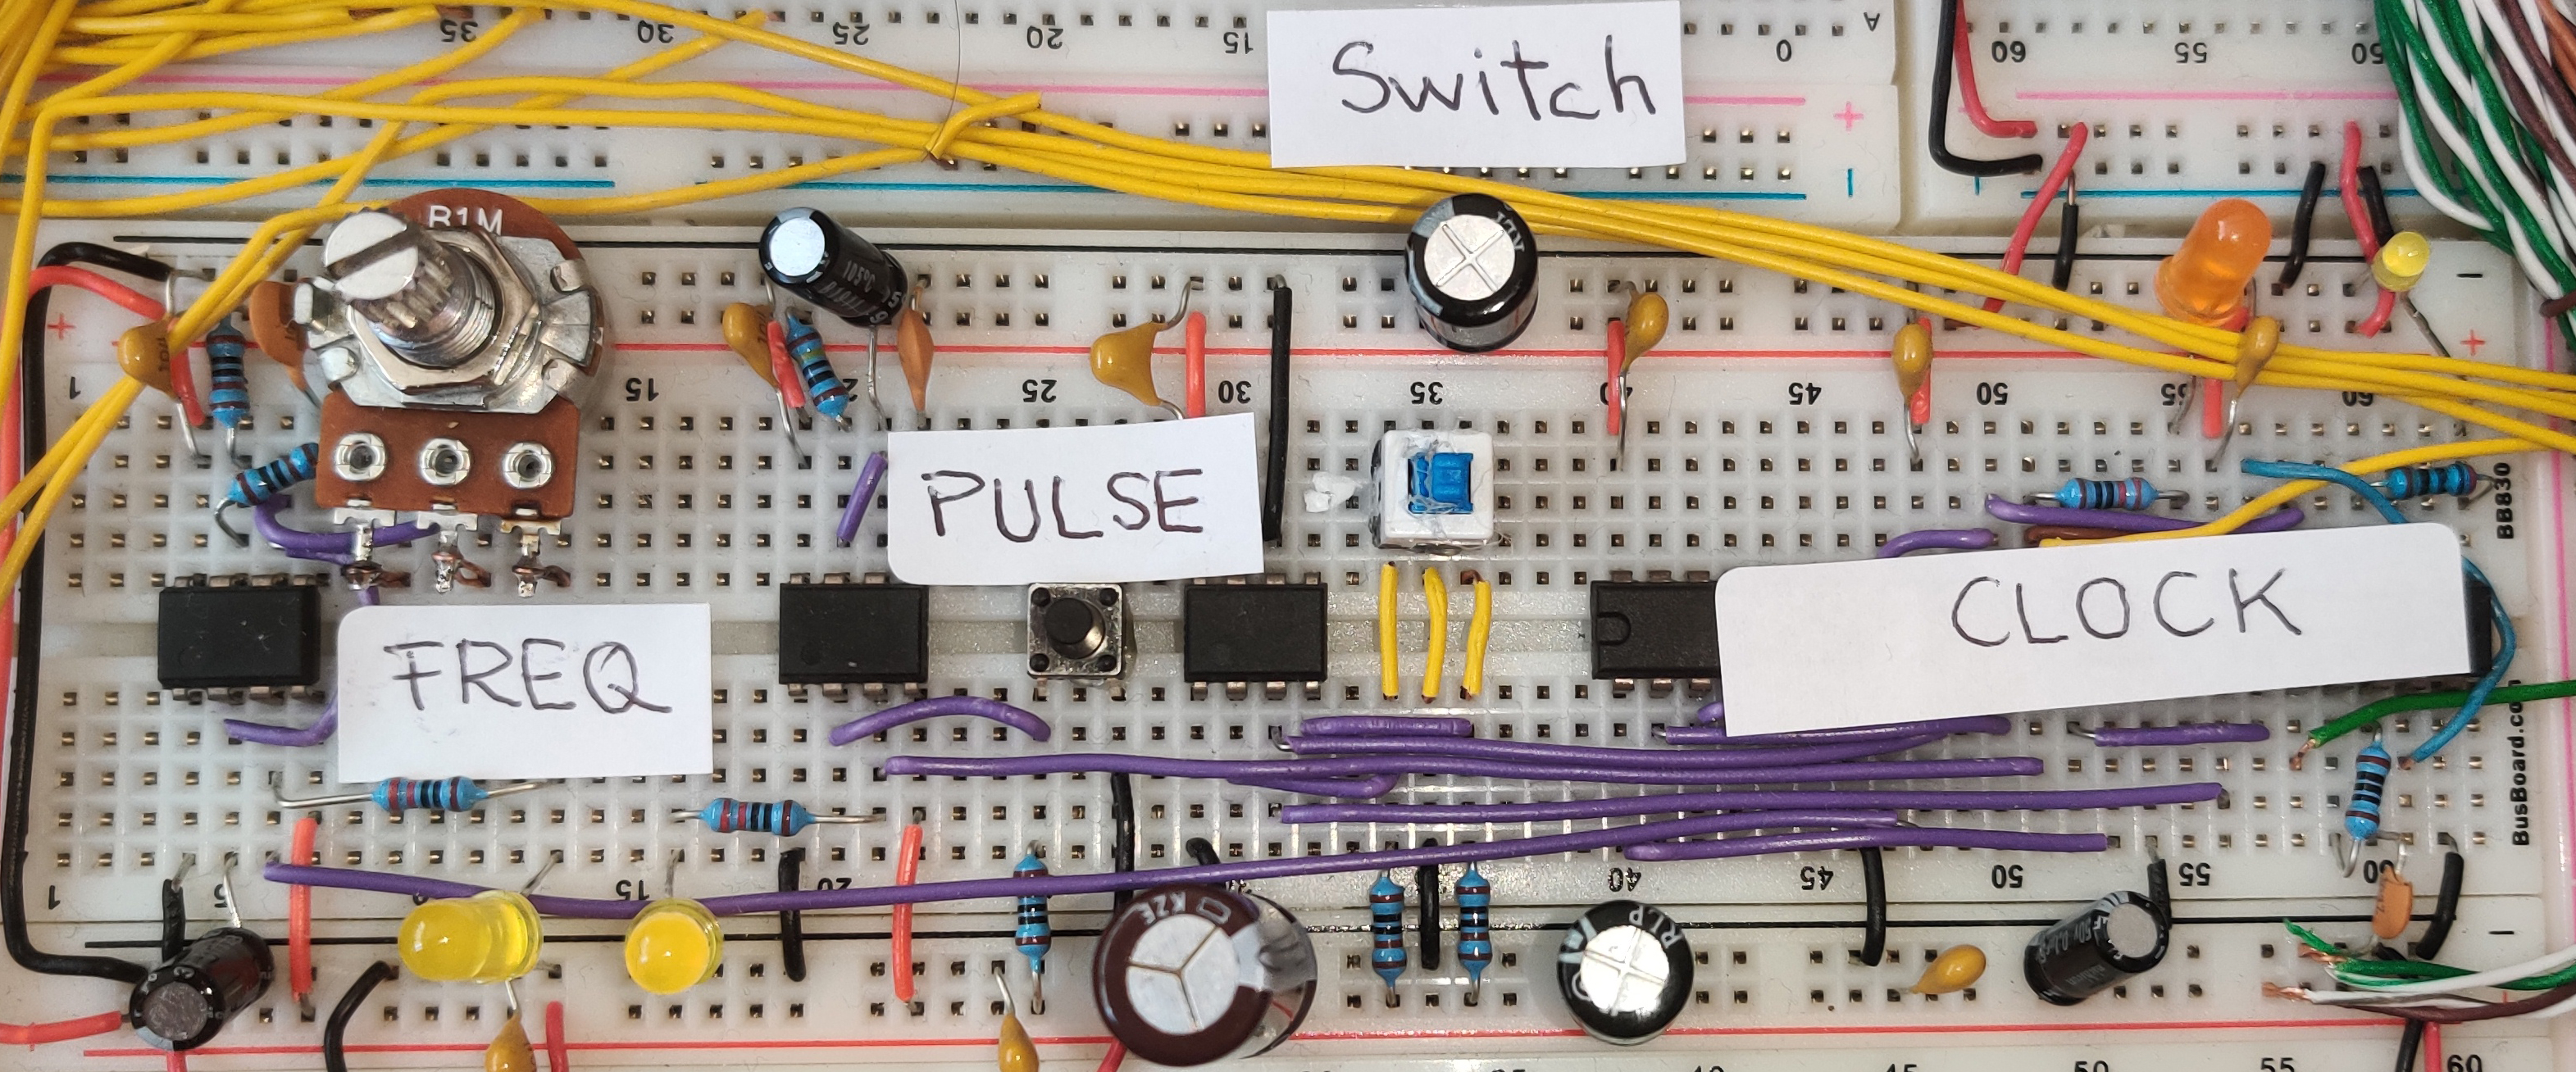
\includegraphics[scale=0.1]{comp/clock}
    \caption{Clock implementation}
    \label{clock-i}
  \end{figure}

  \begin{figure}[h]
    \centering
    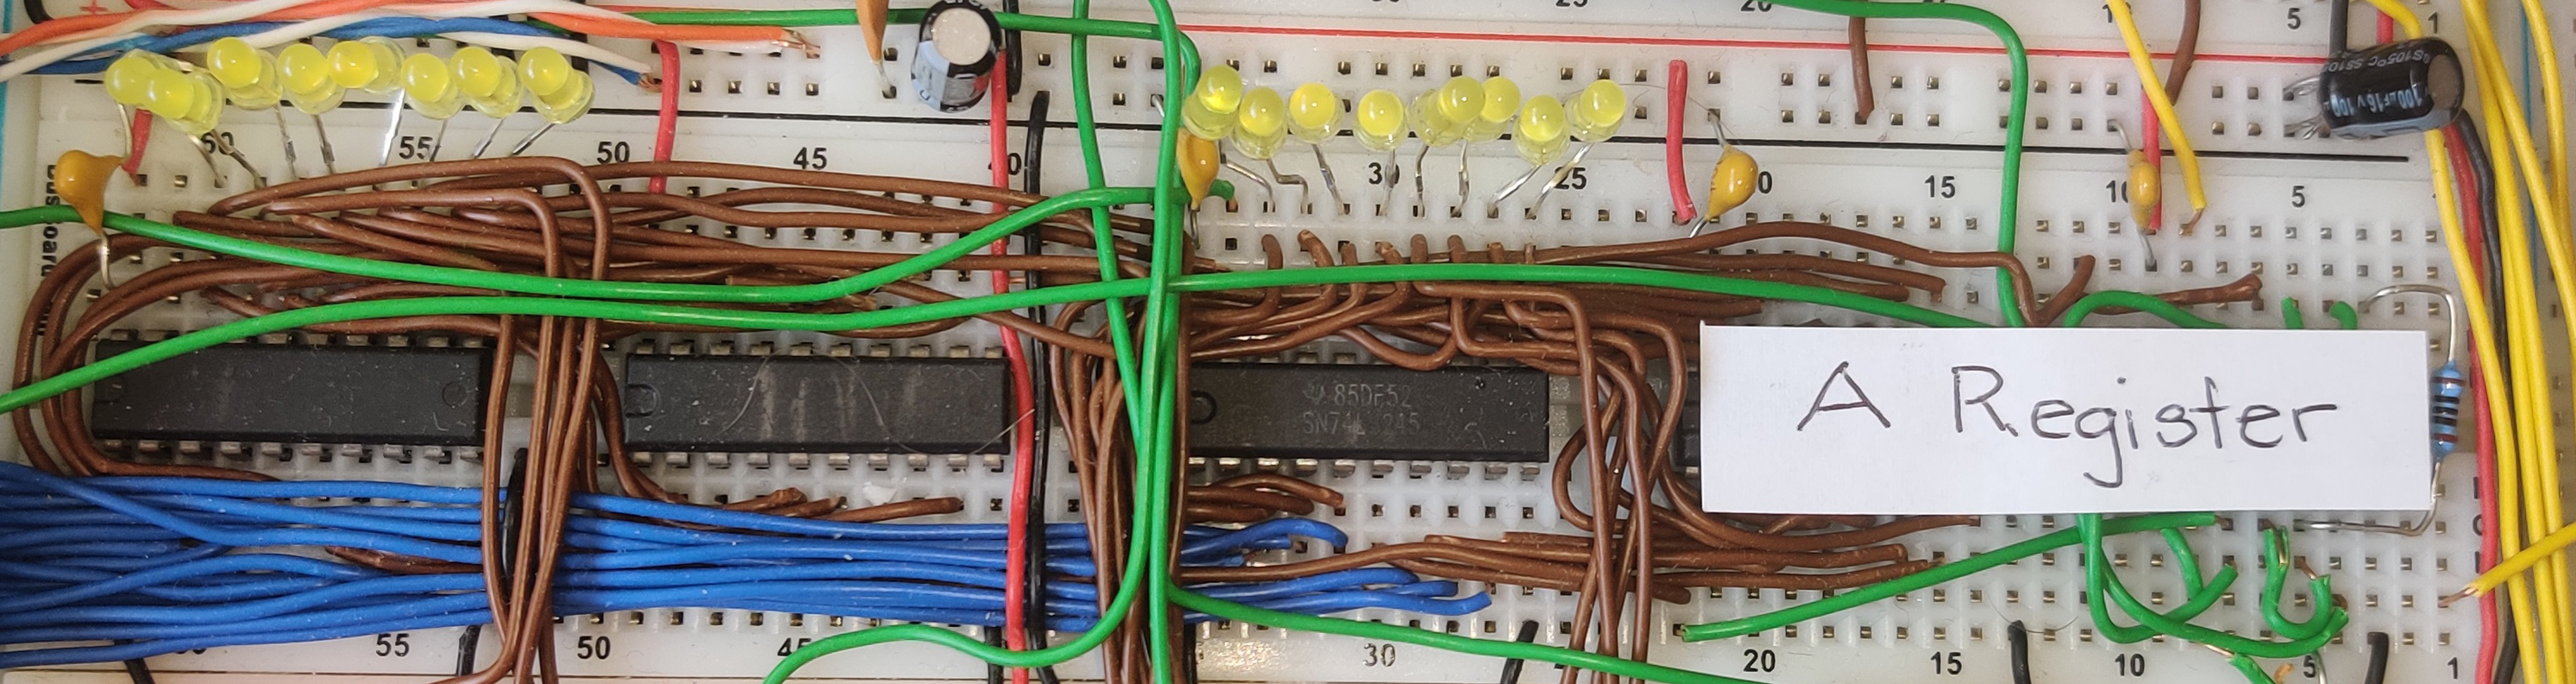
\includegraphics[scale=0.1]{comp/a-reg}
    \caption{A register implementation}
    \label{a-reg-i}
  \end{figure}

  \begin{figure}[h]
    \centering
    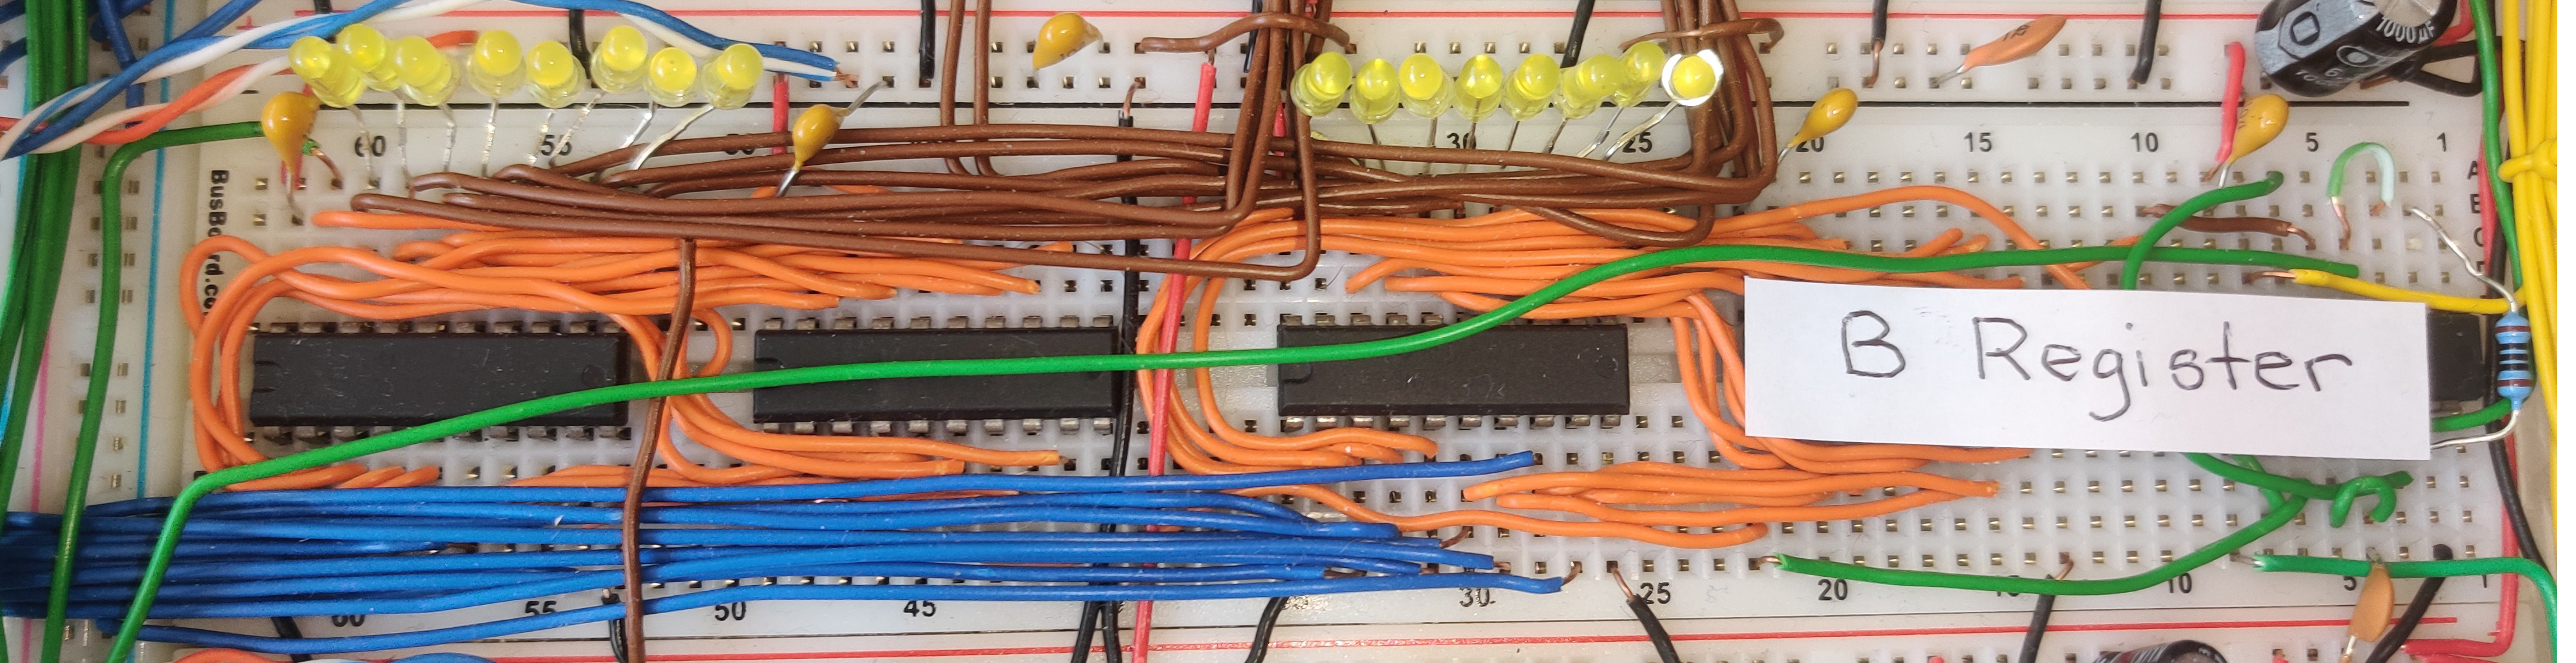
\includegraphics[scale=0.1]{comp/b-reg}
    \caption{B register implementation}
    \label{b-reg-i}
  \end{figure}

  \begin{figure}[h]
    \centering
    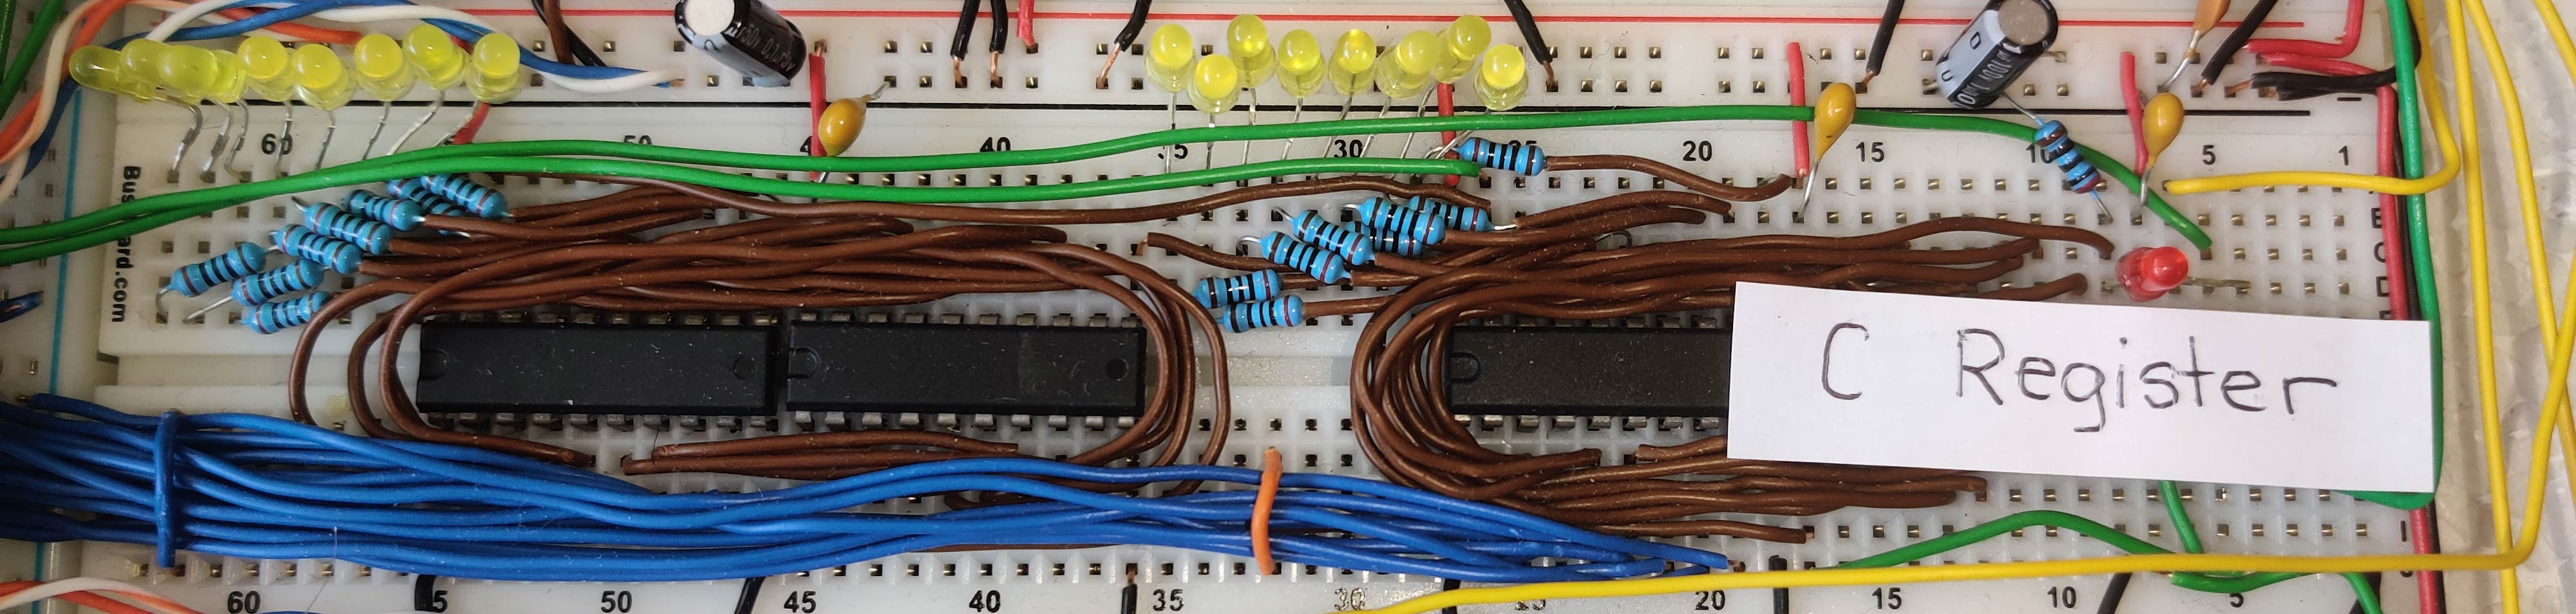
\includegraphics[scale=0.1]{comp/c-reg}
    \caption{C register implementation}
    \label{c-reg-i}
  \end{figure}

  \begin{figure}[h]
    \centering
    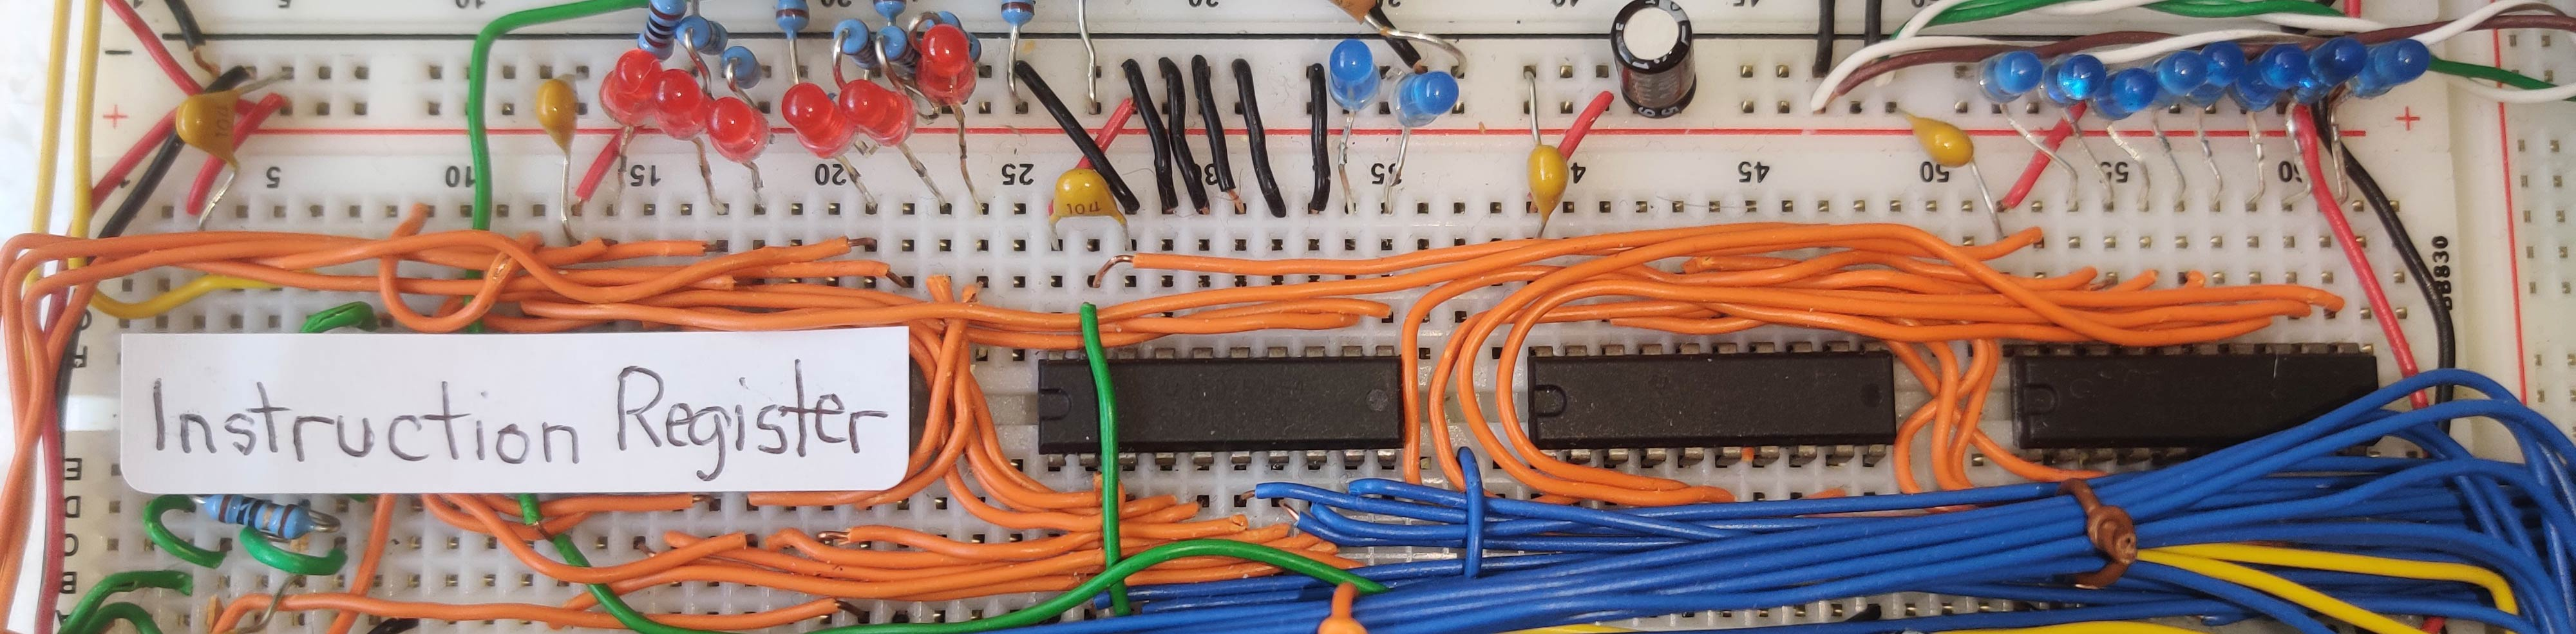
\includegraphics[scale=0.1]{comp/ir}
    \caption{Instruction register implementation}
    \label{ir-i}
  \end{figure}

  \begin{figure}[h]
    \centering
    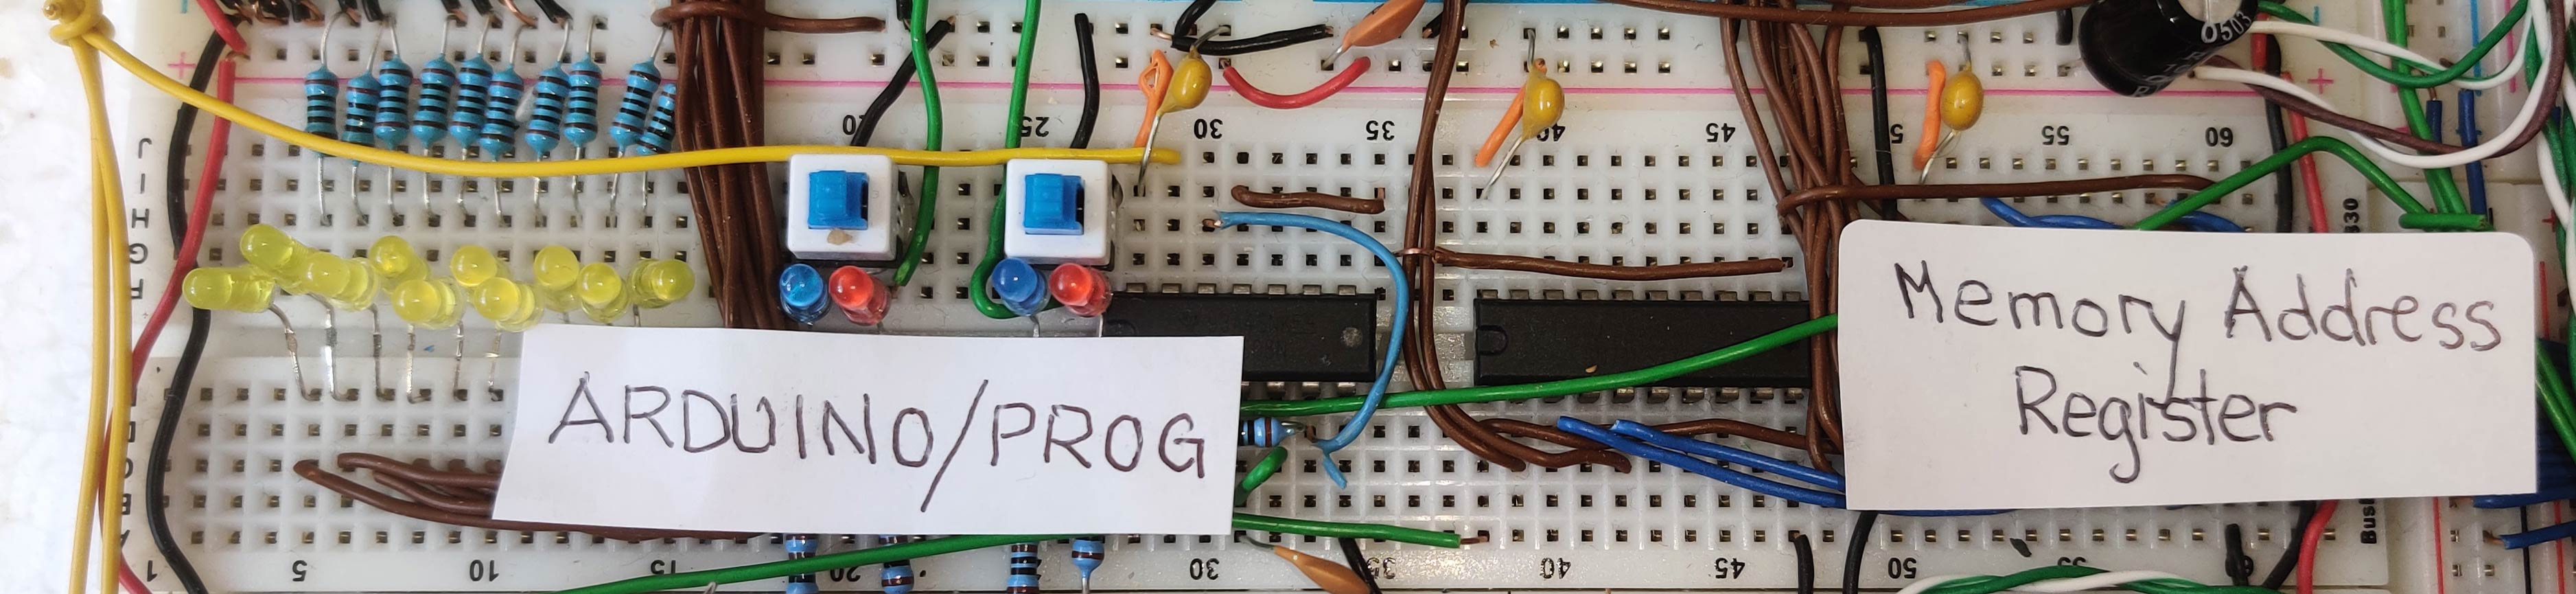
\includegraphics[scale=0.1]{comp/mar}
    \caption{Memory address register implementation}
    \label{mar-i}
  \end{figure}

  \begin{figure}[h]
    \centering
    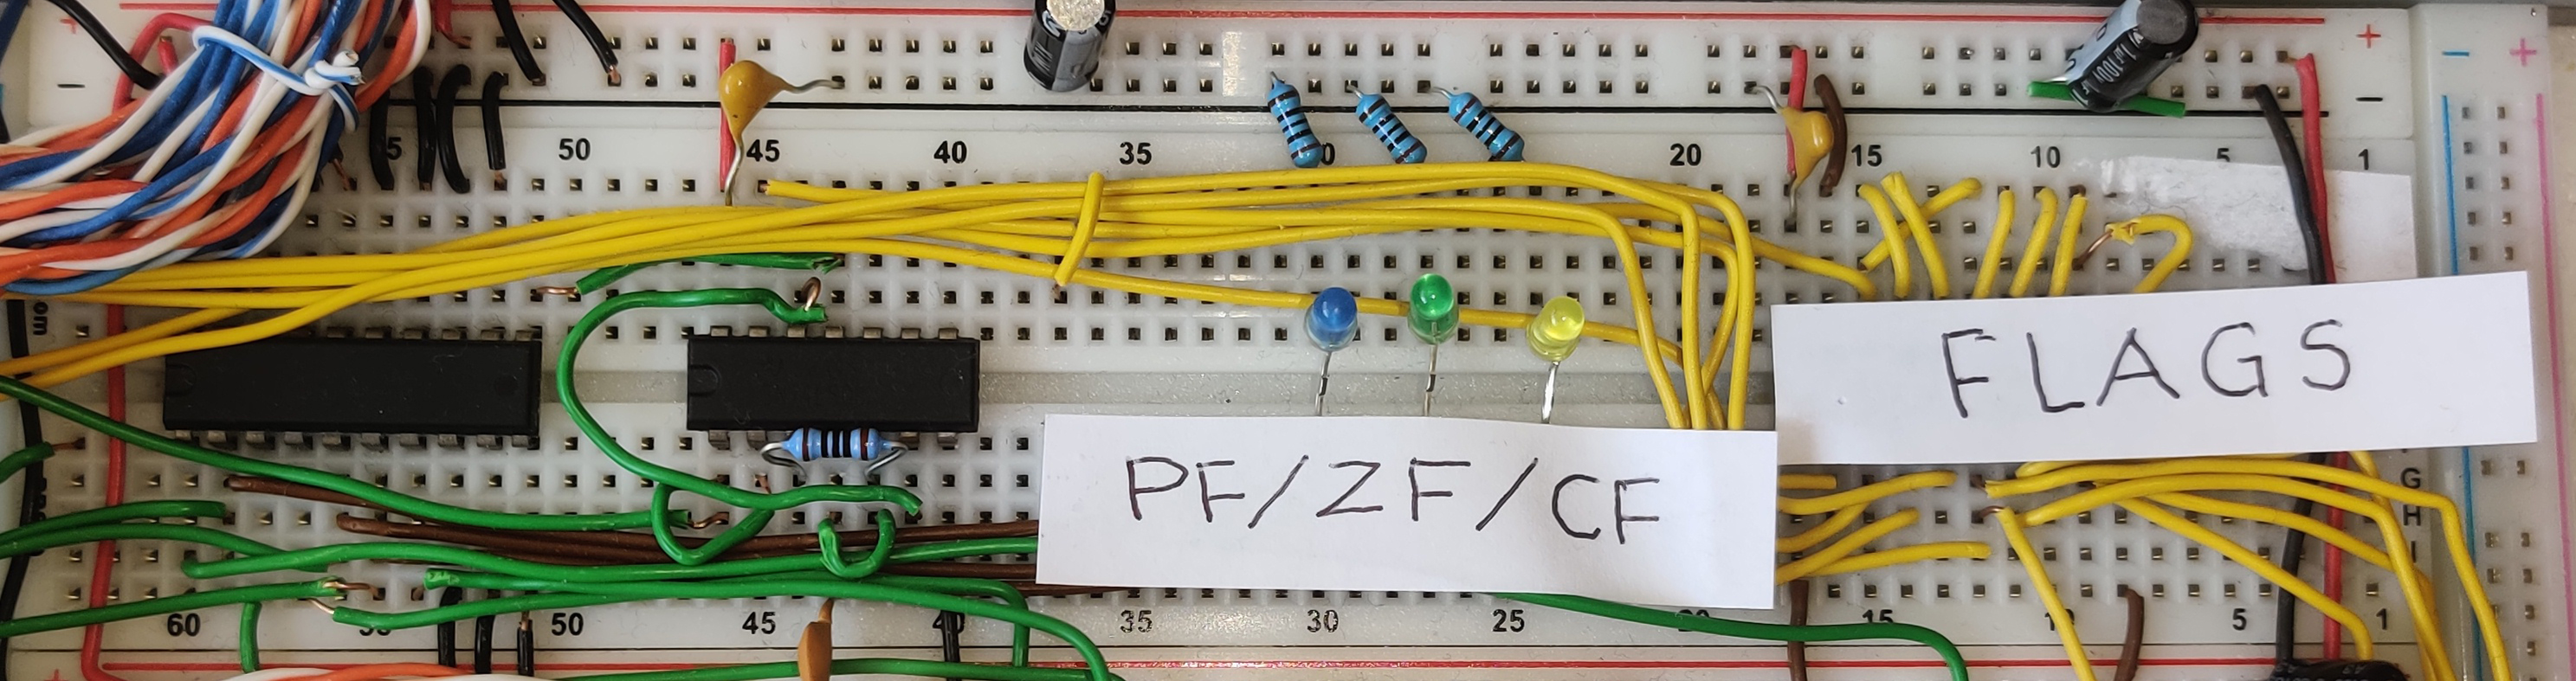
\includegraphics[scale=0.1]{comp/flags}
    \caption{Flags register implementation}
    \label{flags-i}
  \end{figure}

  \begin{figure}[h]
    \centering
    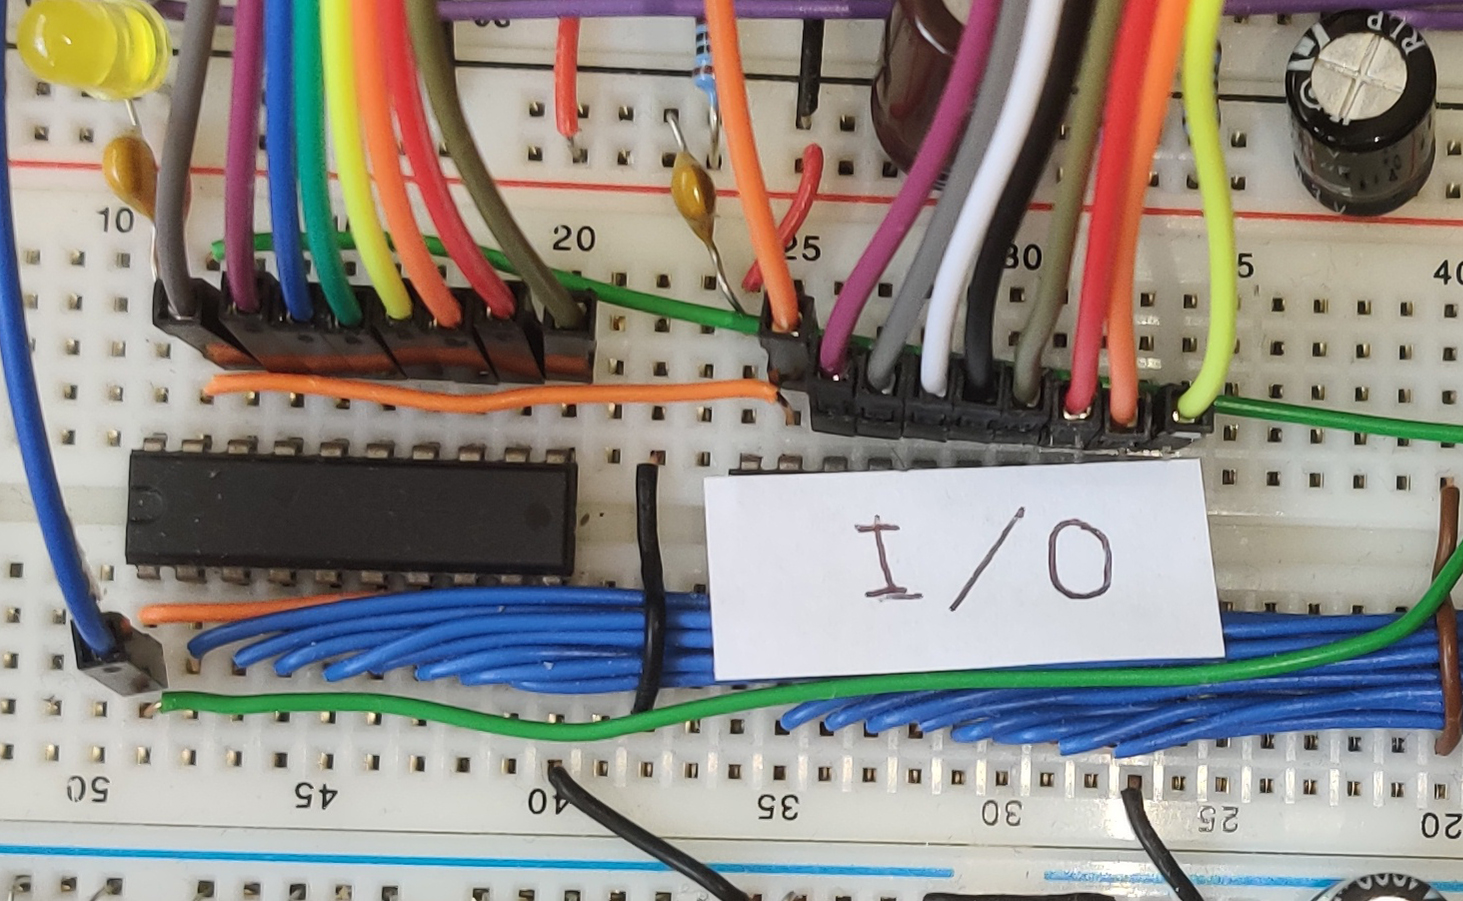
\includegraphics[scale=0.1]{comp/io}
    \caption{Input/Output implementation}
    \label{io-i}
  \end{figure}

  \begin{figure}[h]
    \centering
    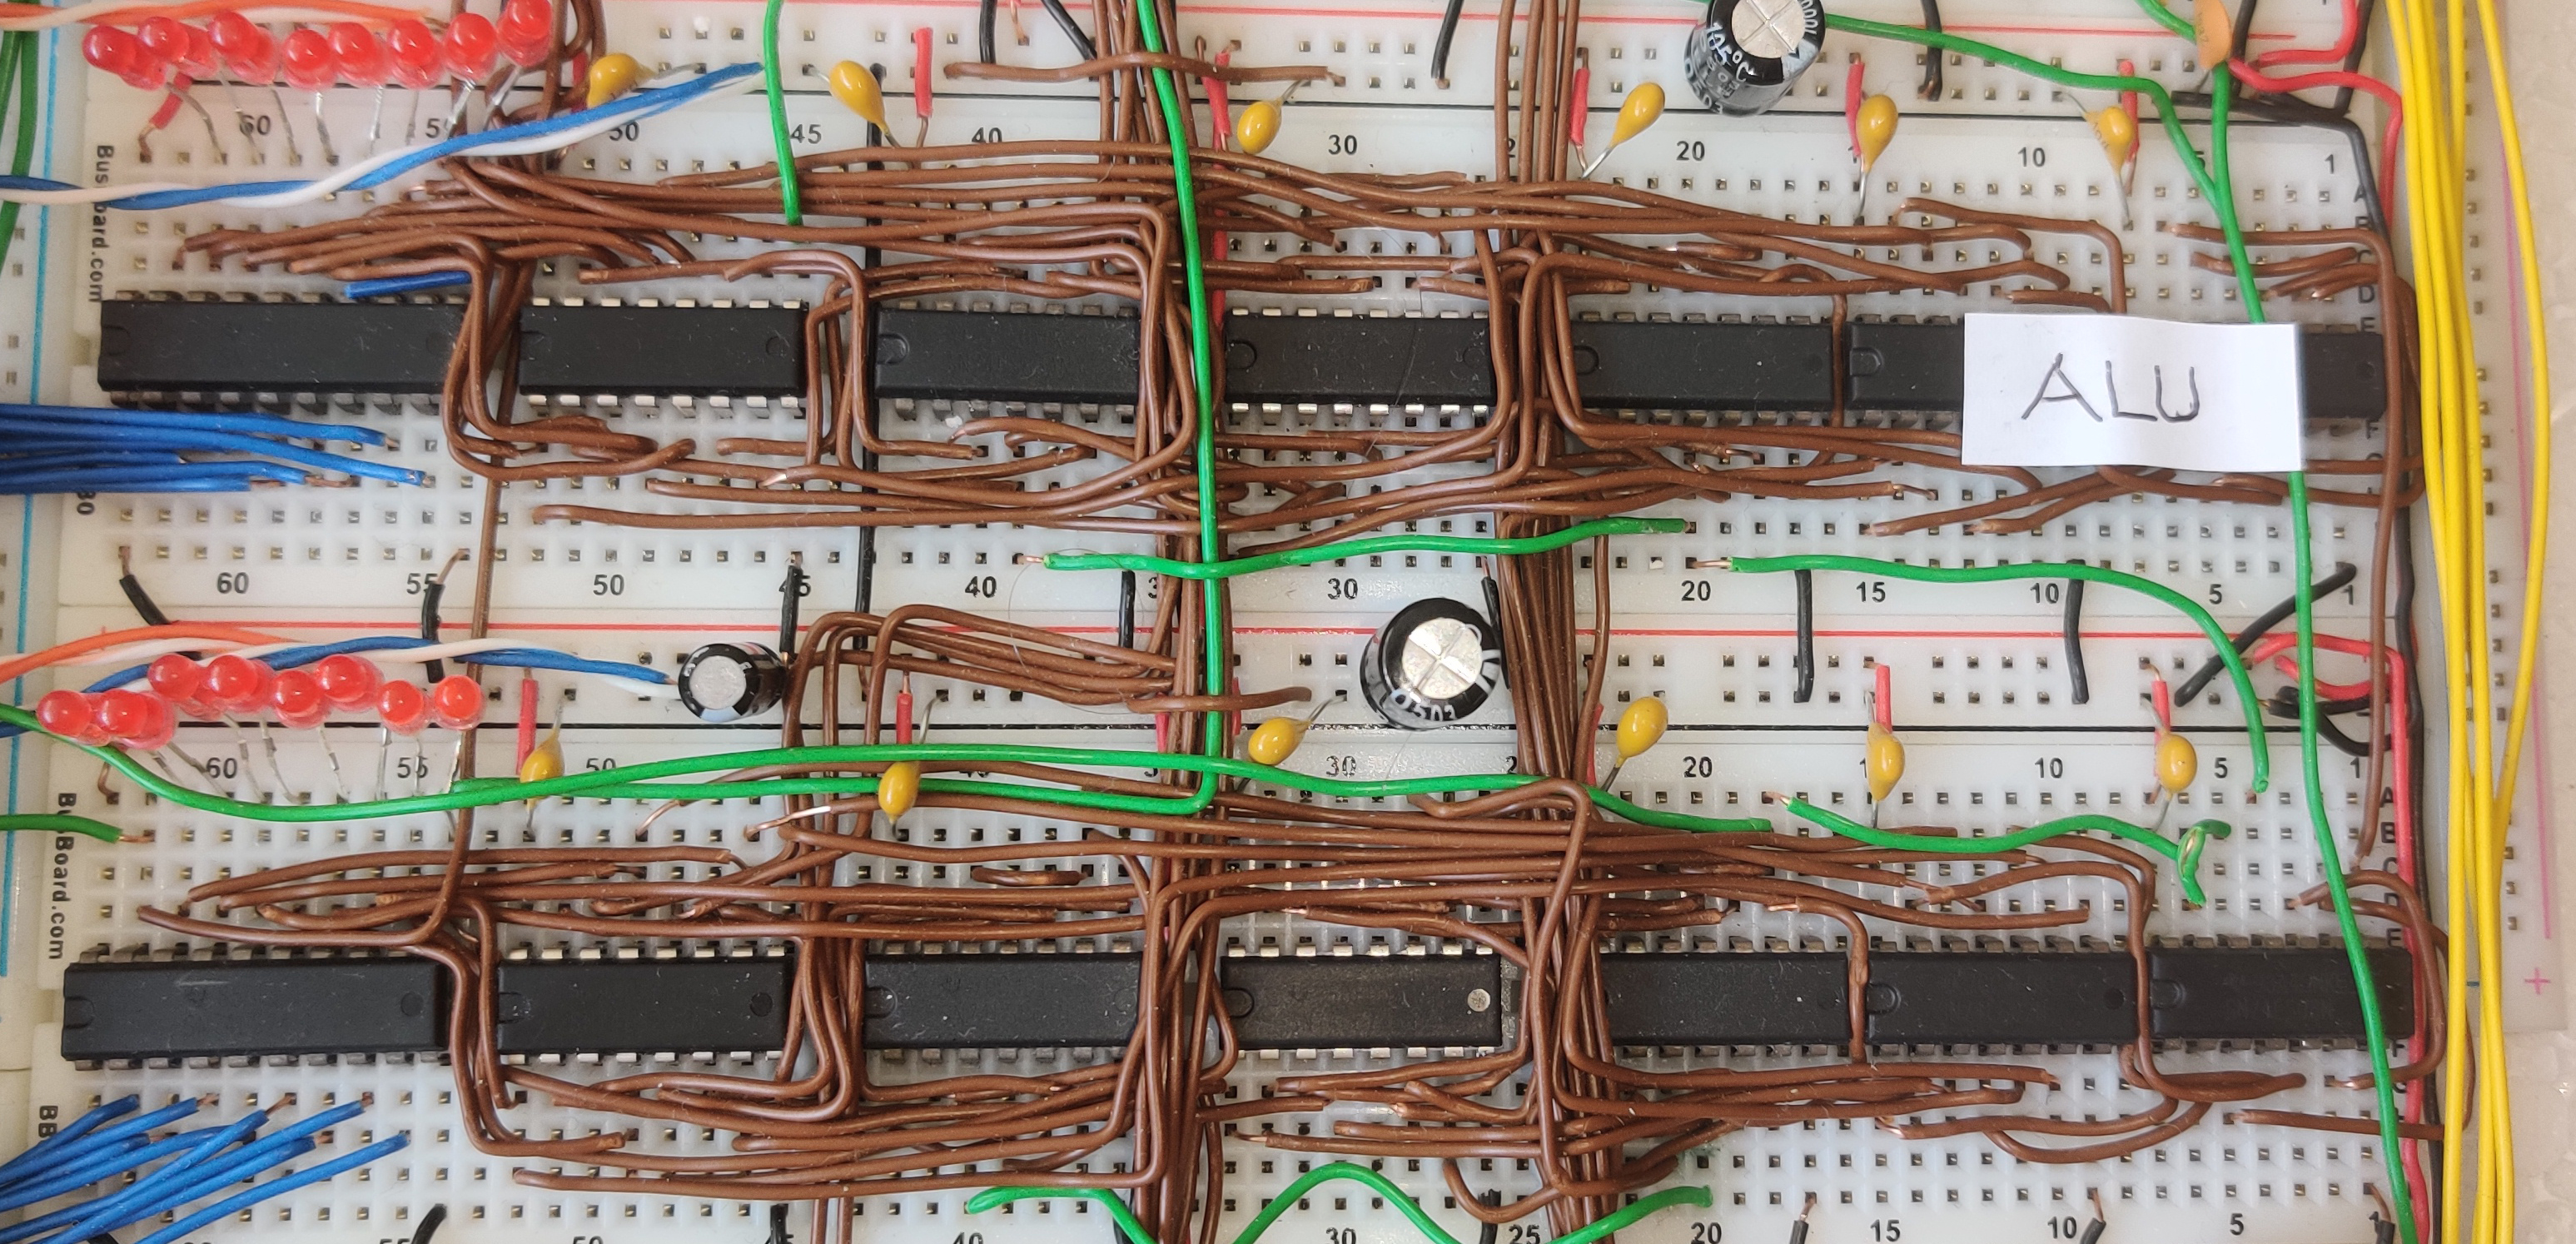
\includegraphics[scale=0.1]{comp/alu}
    \caption{Arithmetic-Logic Unit implementation}
    \label{alu-i}
  \end{figure}

  \begin{figure}[h]
    \centering
    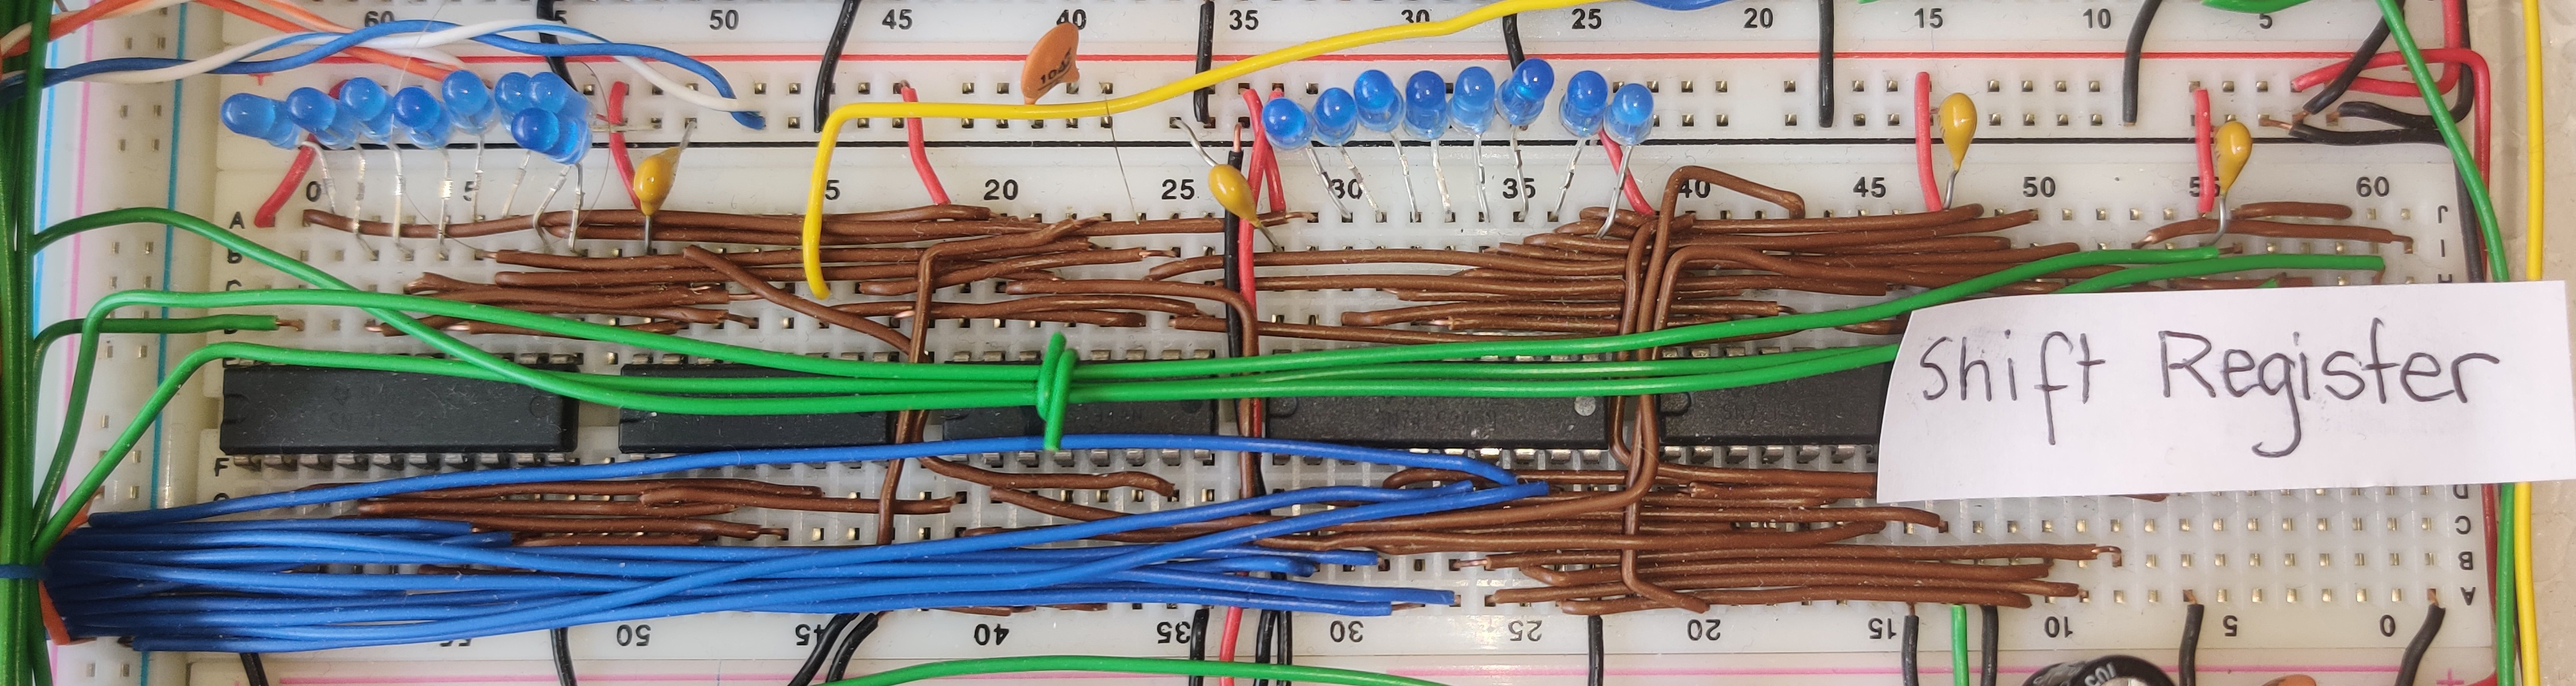
\includegraphics[scale=0.1]{comp/shift-reg}
    \caption{Shift Register implementation}
    \label{shift-reg-i}
  \end{figure}

  \begin{figure}[h]
    \centering
    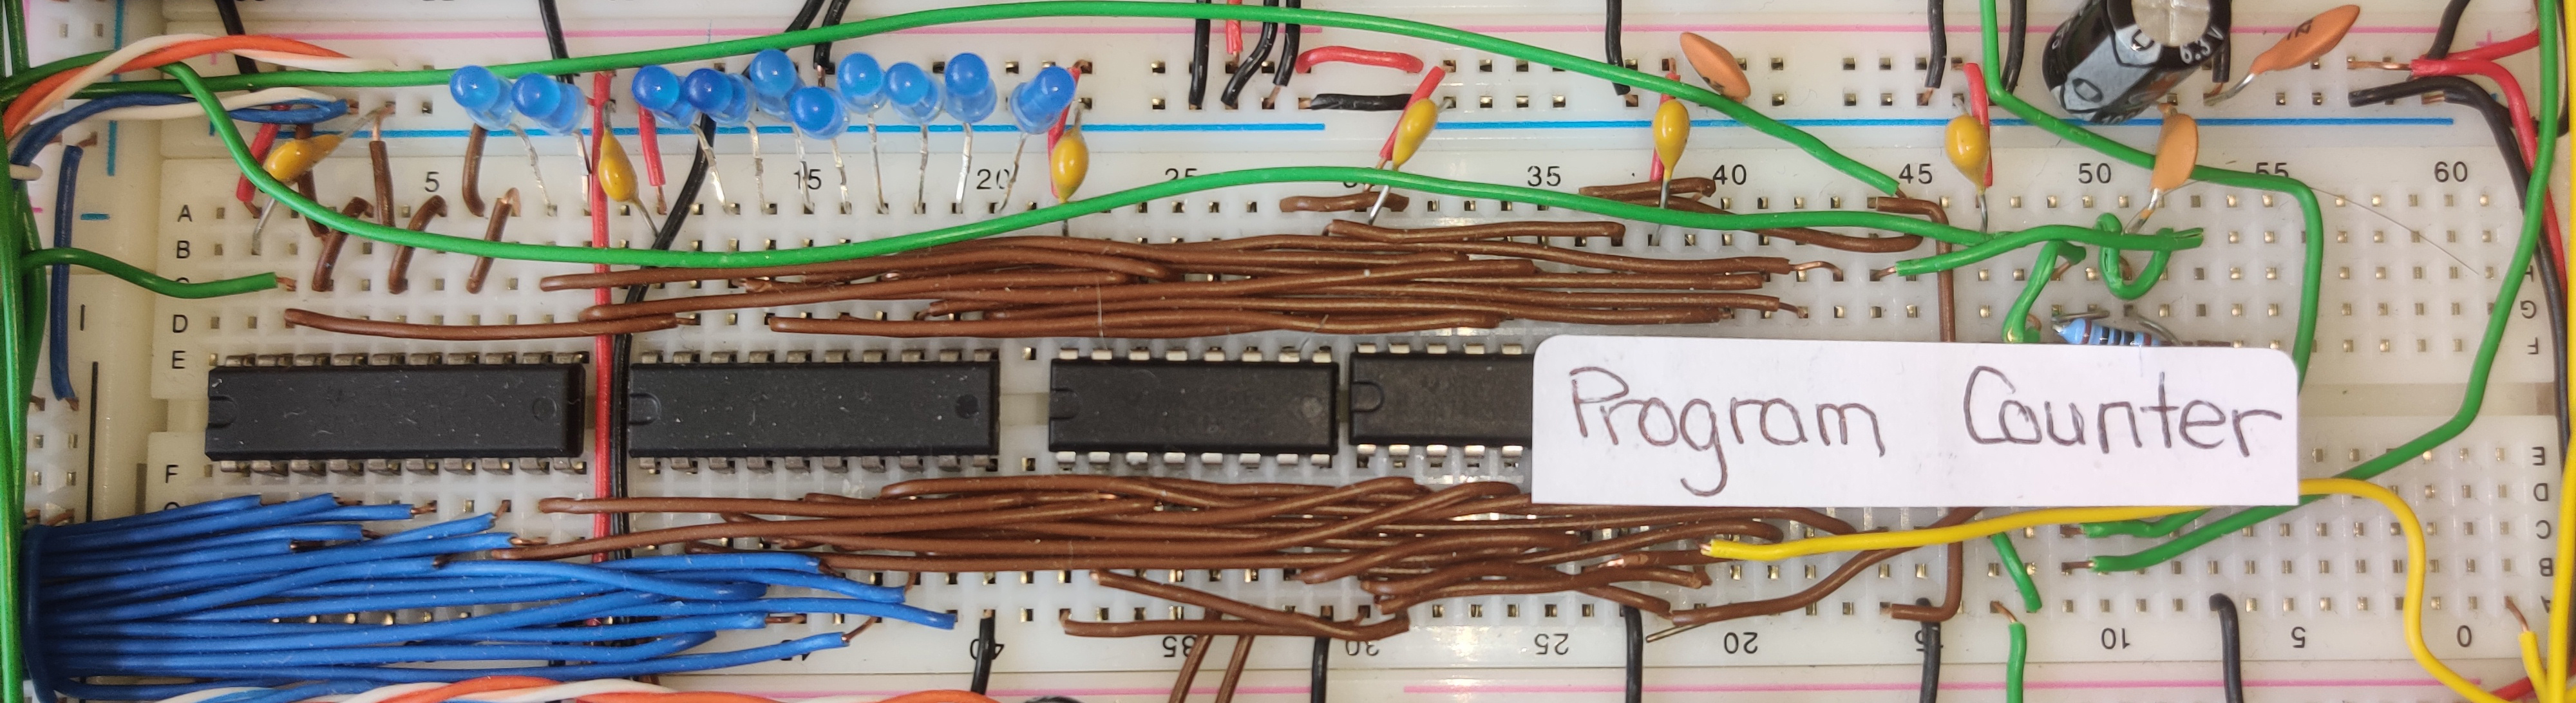
\includegraphics[scale=0.1]{comp/pc}
    \caption{Program Counter implementation}
    \label{pc-i}
  \end{figure}

  \begin{figure}[h]
    \centering
    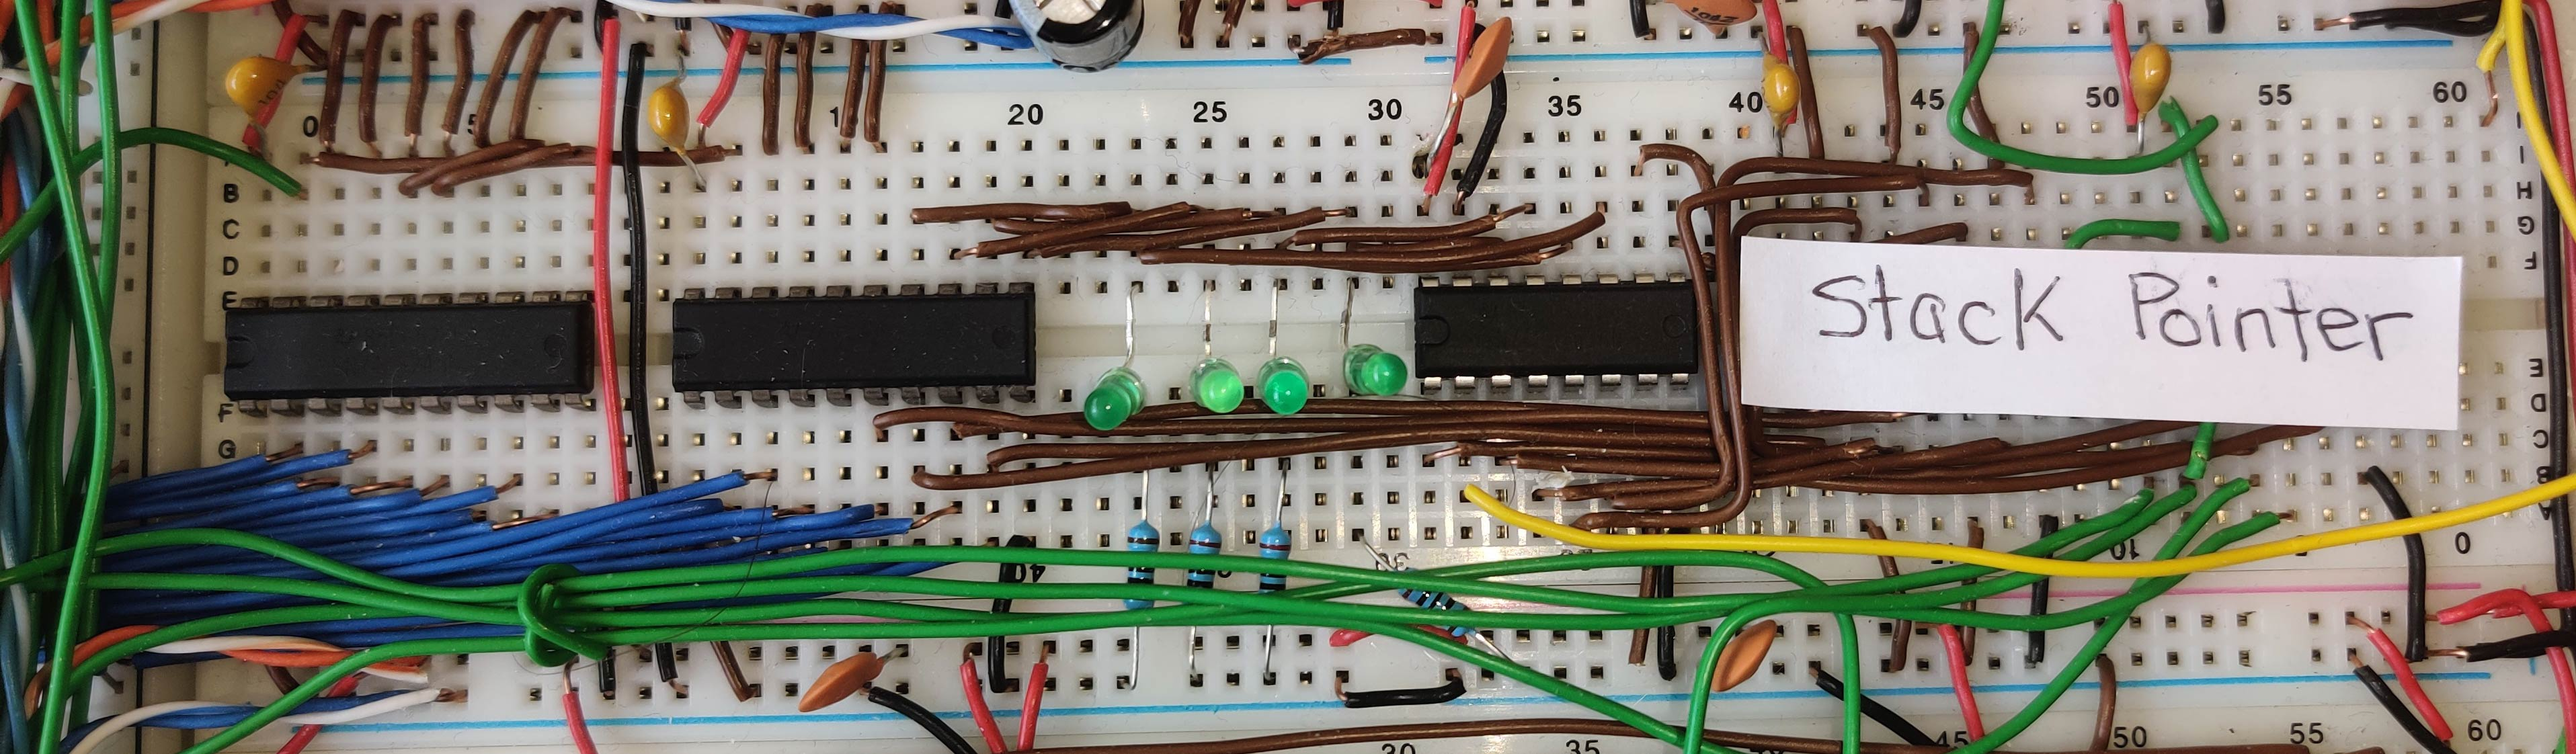
\includegraphics[scale=0.1]{comp/sp}
    \caption{Stack Pointer implementation}
    \label{sp-i}
  \end{figure}

  \begin{figure}[h]
    \centering
    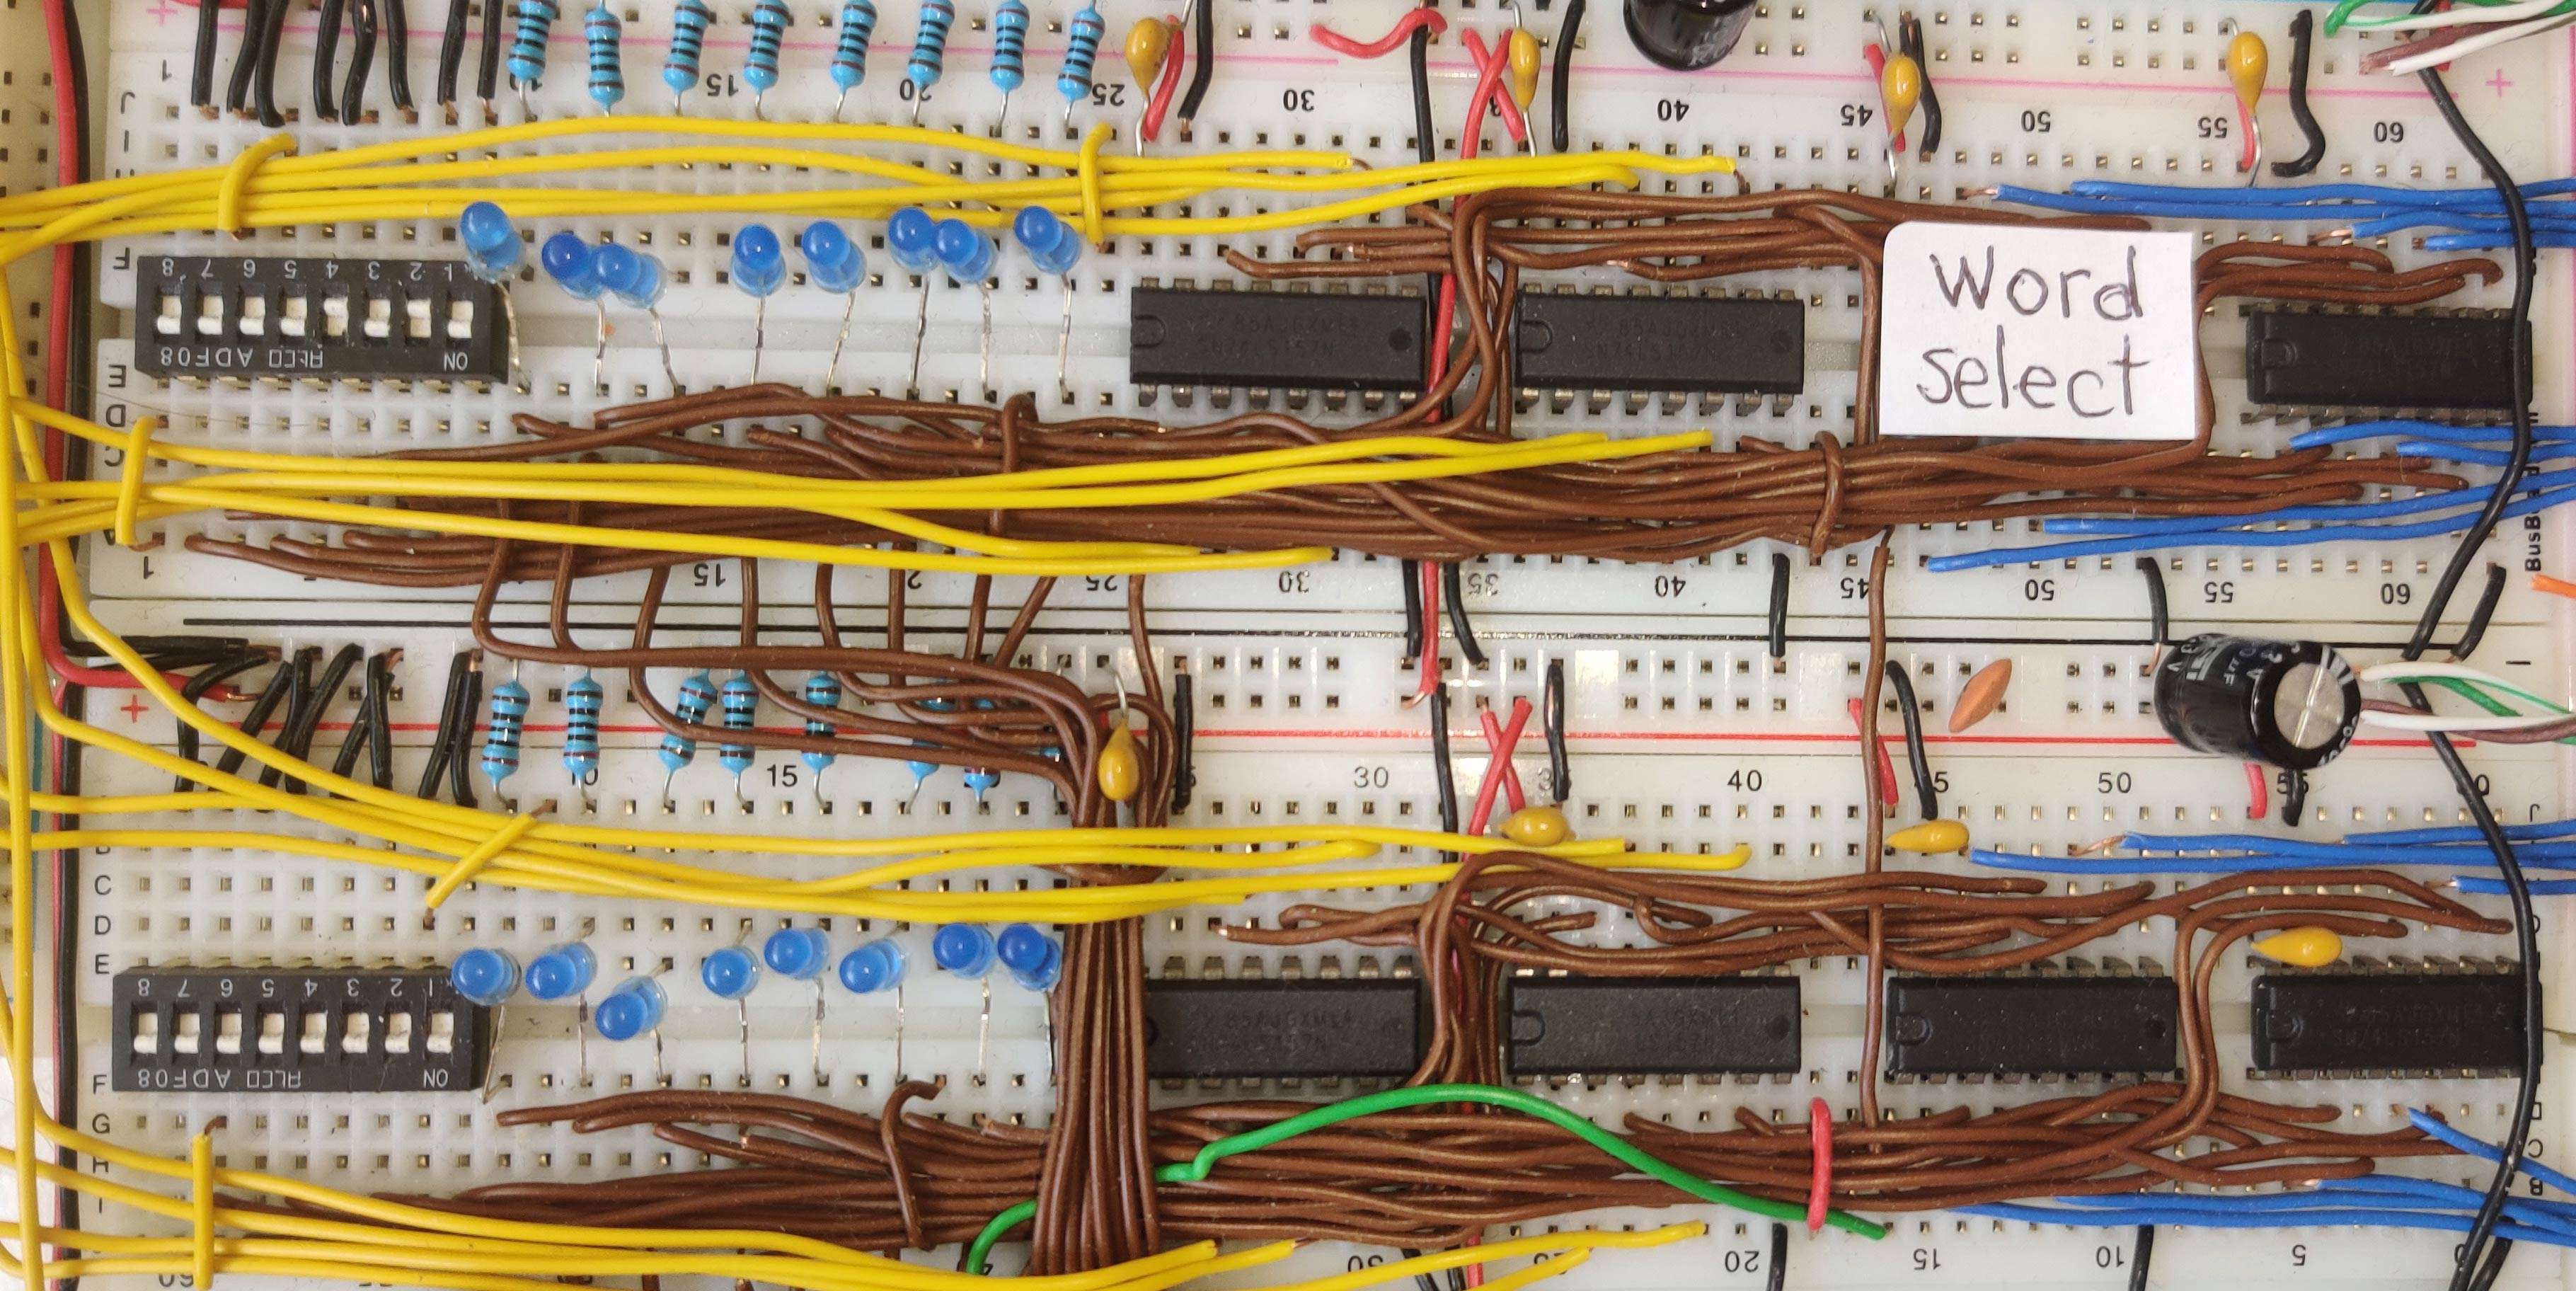
\includegraphics[scale=0.1]{comp/word-select}
    \caption{Word selector implementation}
    \label{word-select-i}
  \end{figure}

  \begin{figure}[h]
    \centering
    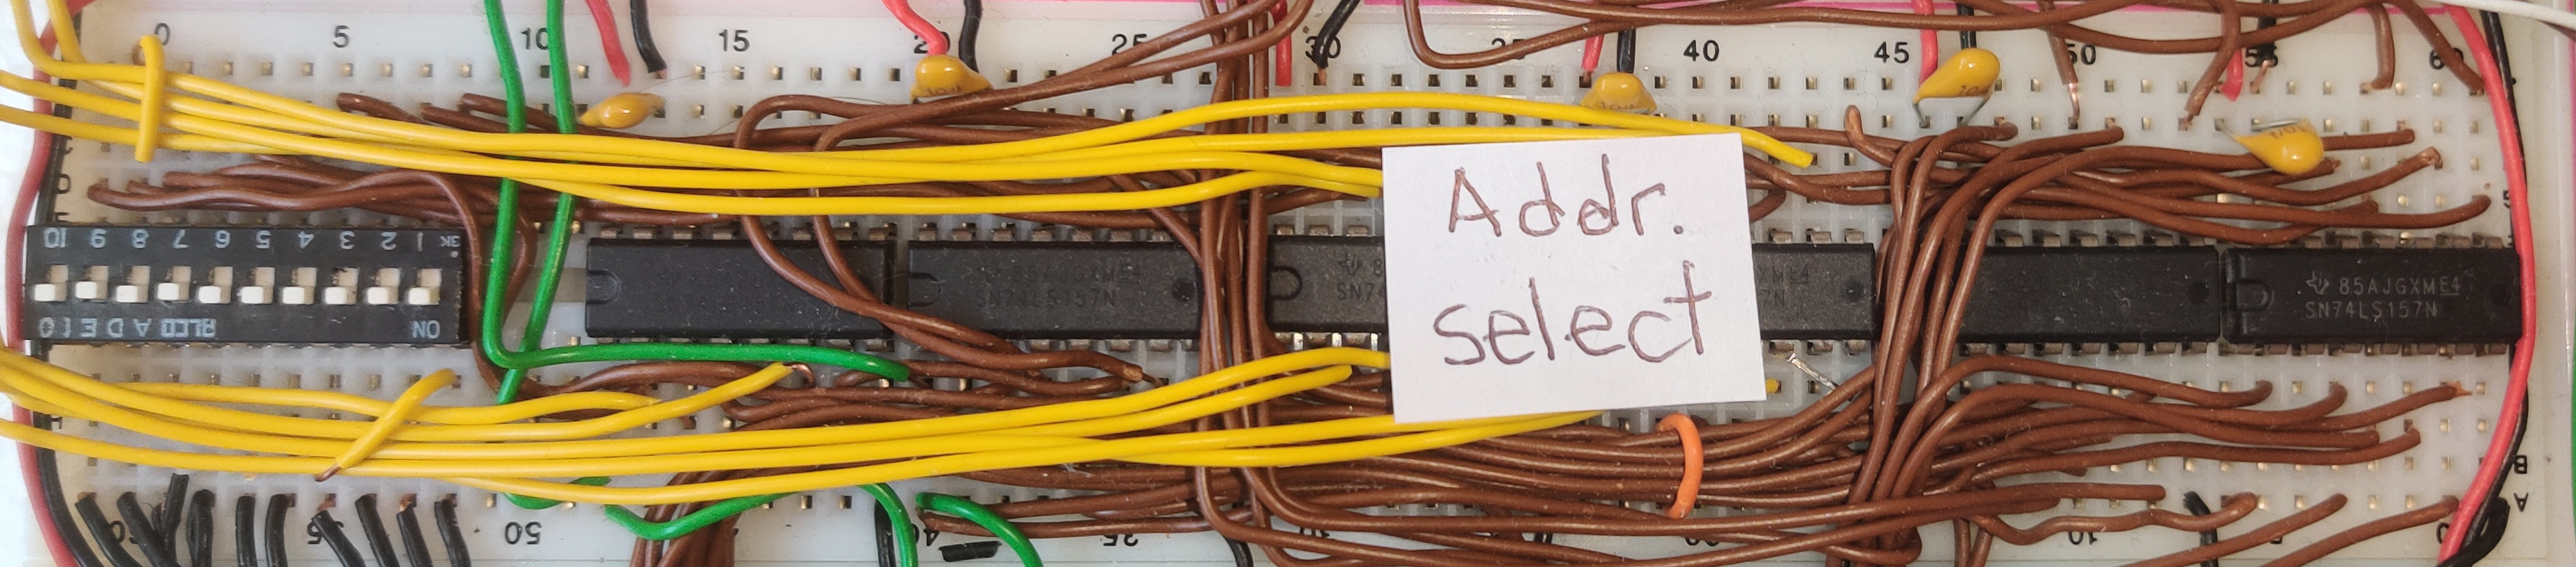
\includegraphics[scale=0.1]{comp/addr-select}
    \caption{Address selector implementation}
    \label{addr-select-i}
  \end{figure}

  \begin{figure}[h]
    \centering
    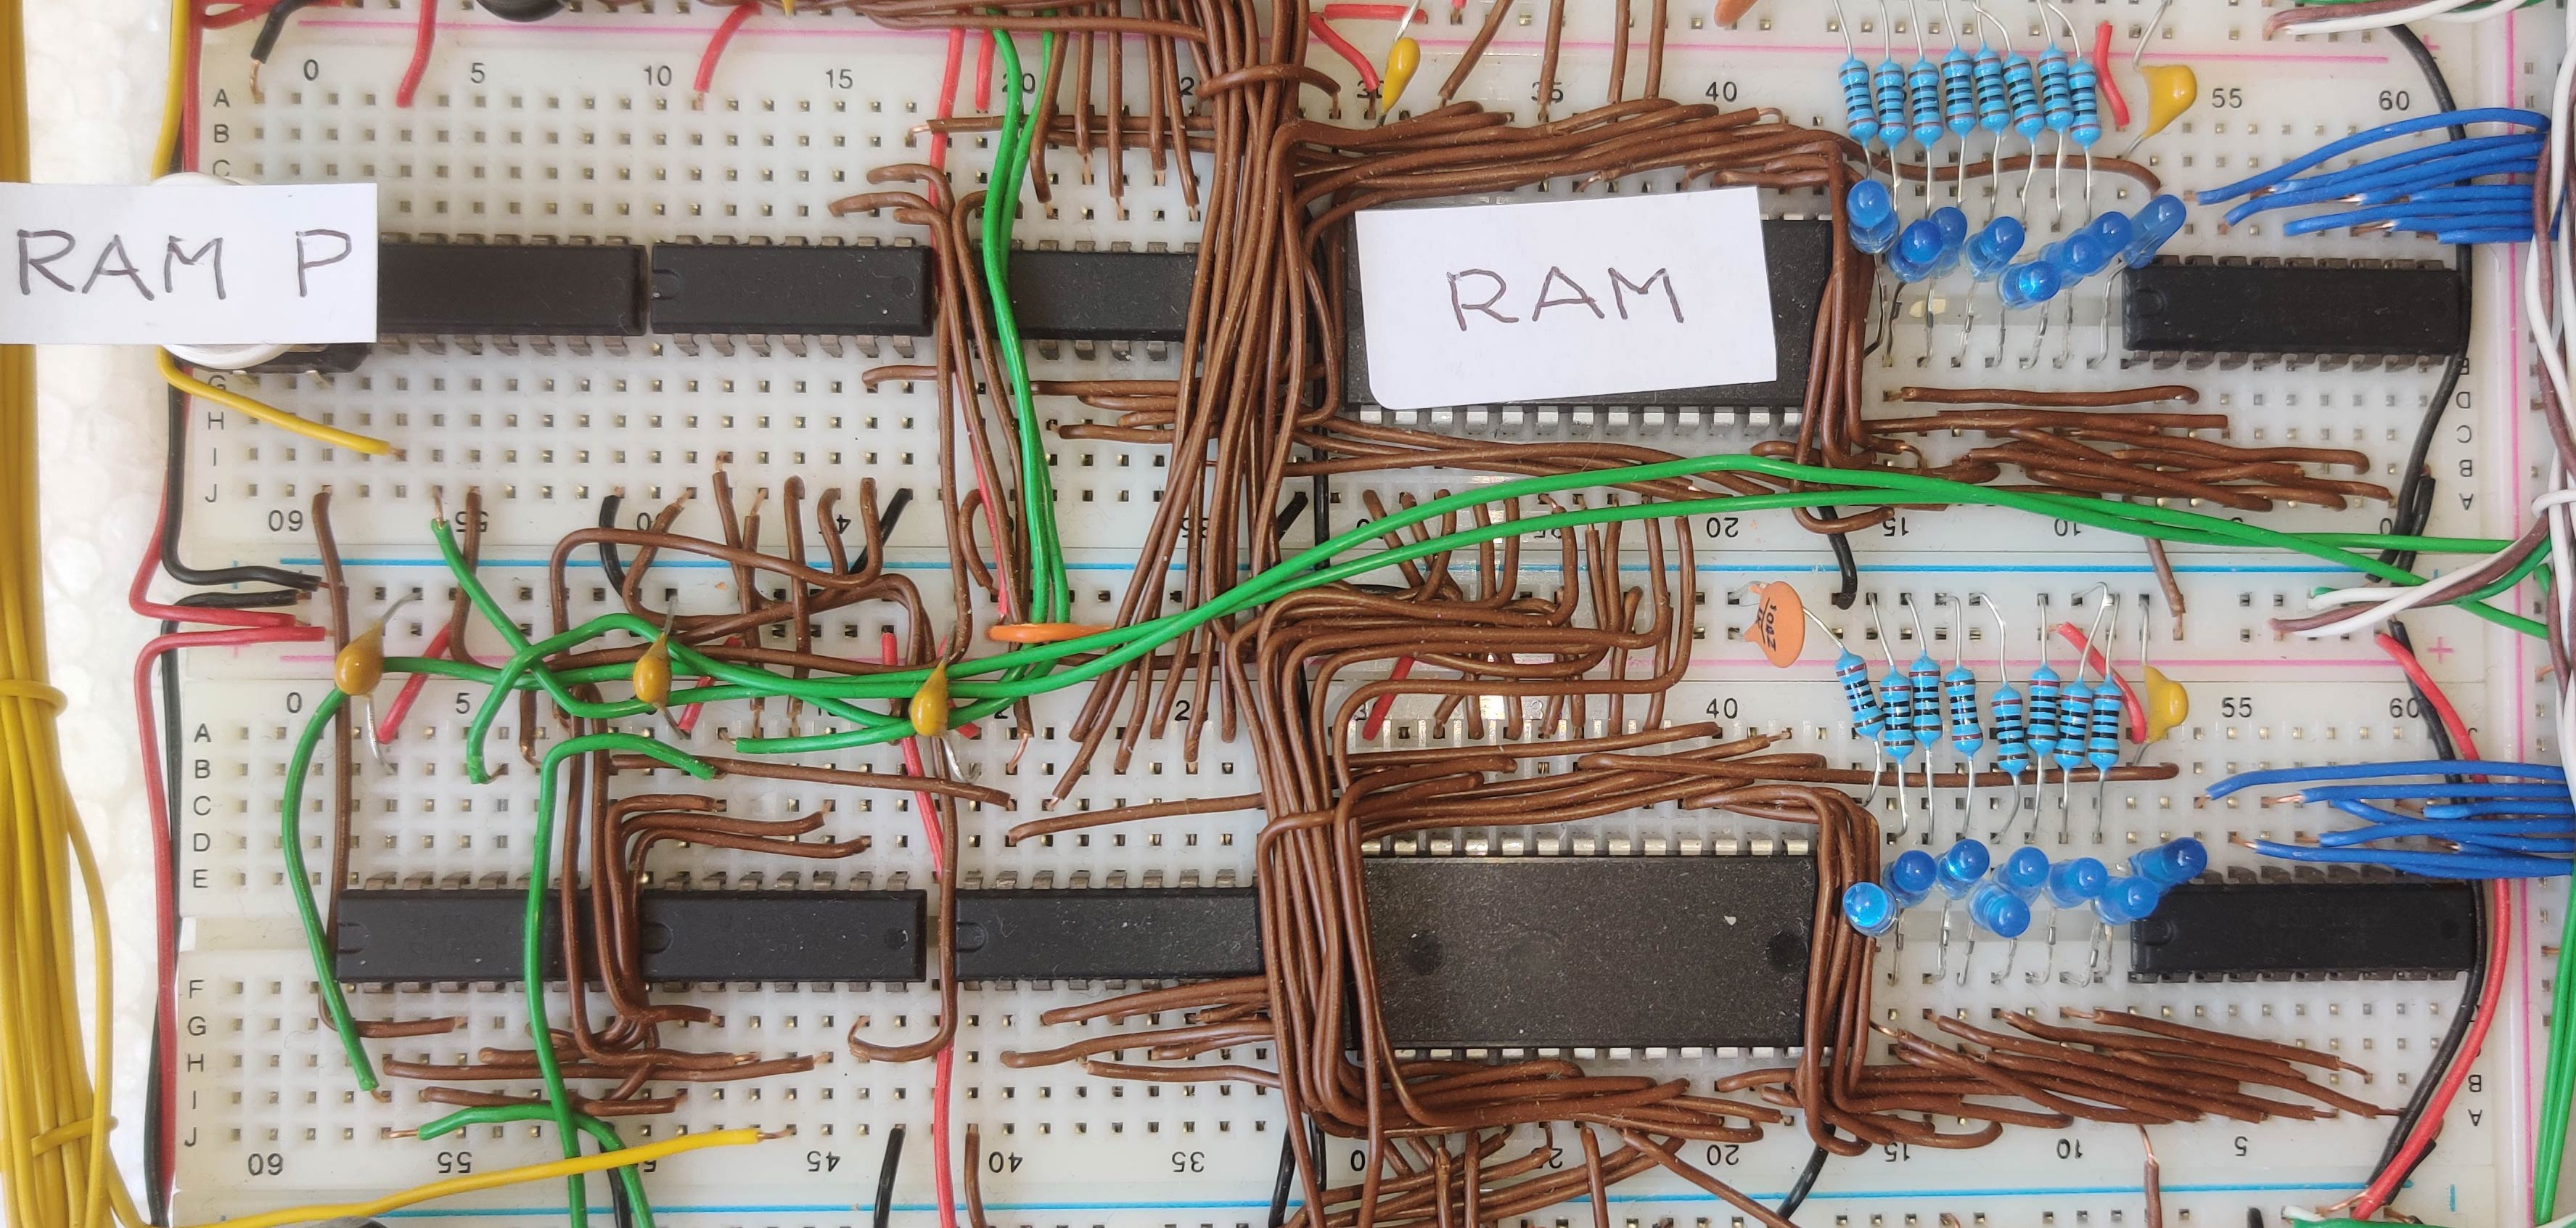
\includegraphics[scale=0.1]{comp/ram}
    \caption{Random Access Memory implementation}
    \label{ram-i}
  \end{figure}

  \begin{figure}[h]
    \centering
    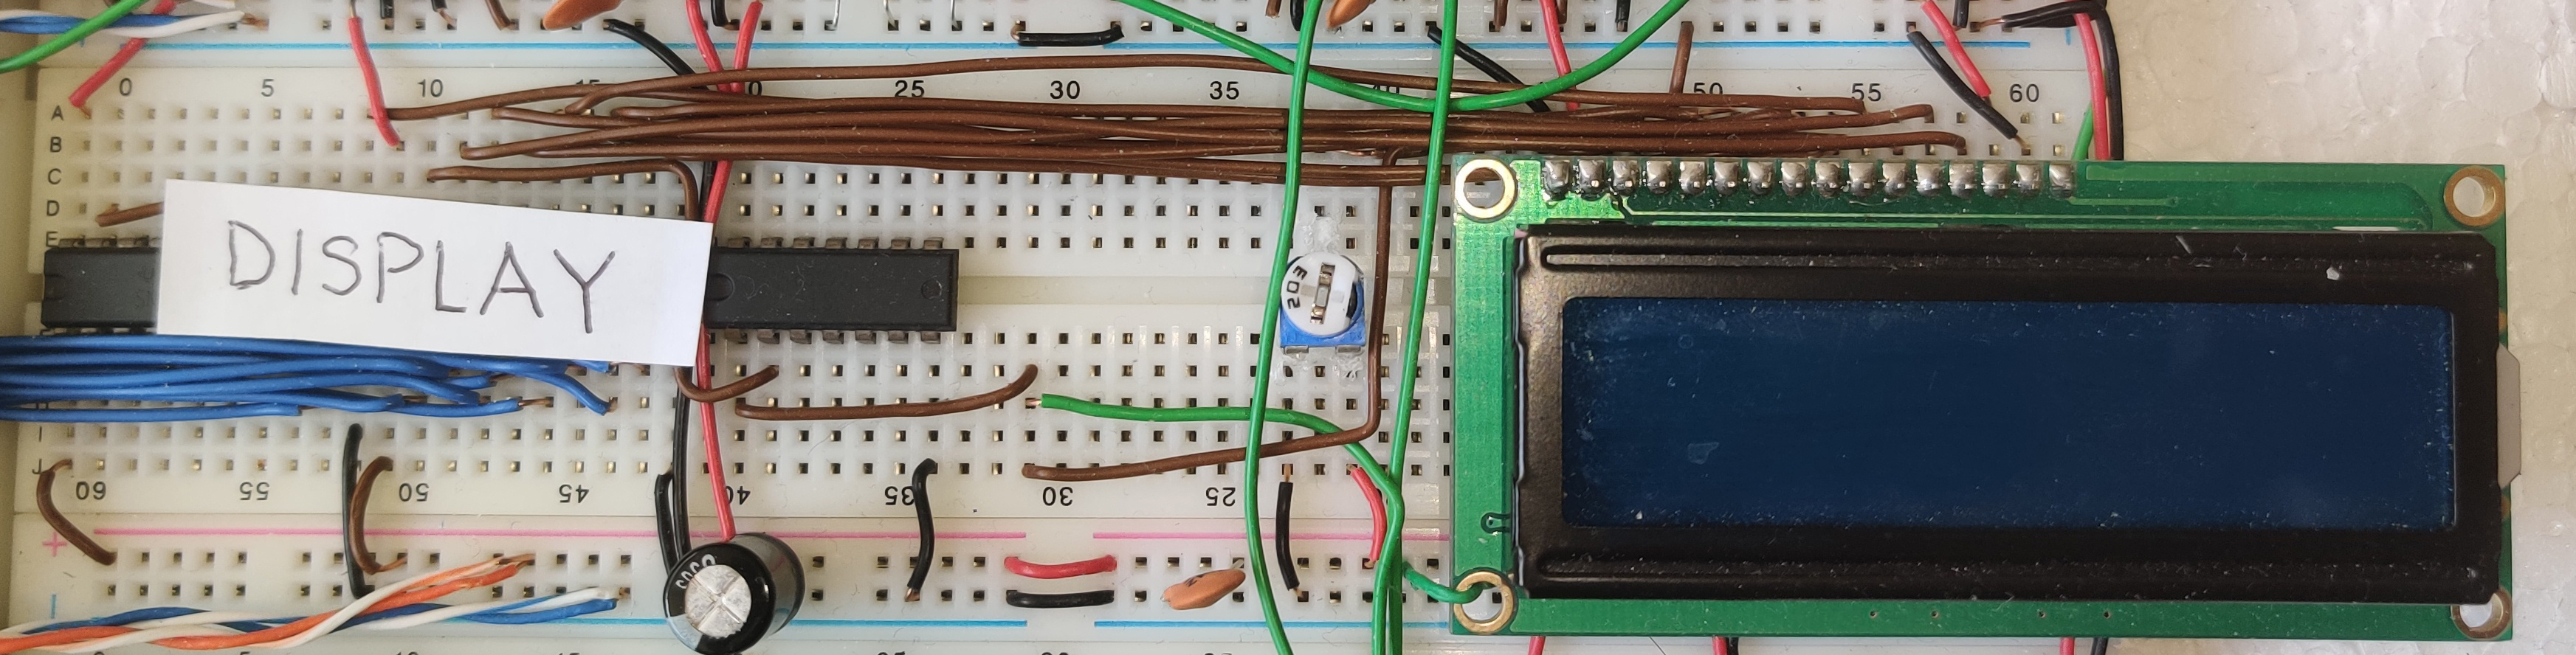
\includegraphics[scale=0.1]{comp/display}
    \caption{Display implementation}
    \label{display-i}
  \end{figure}

  \begin{figure}[h]
    \centering
    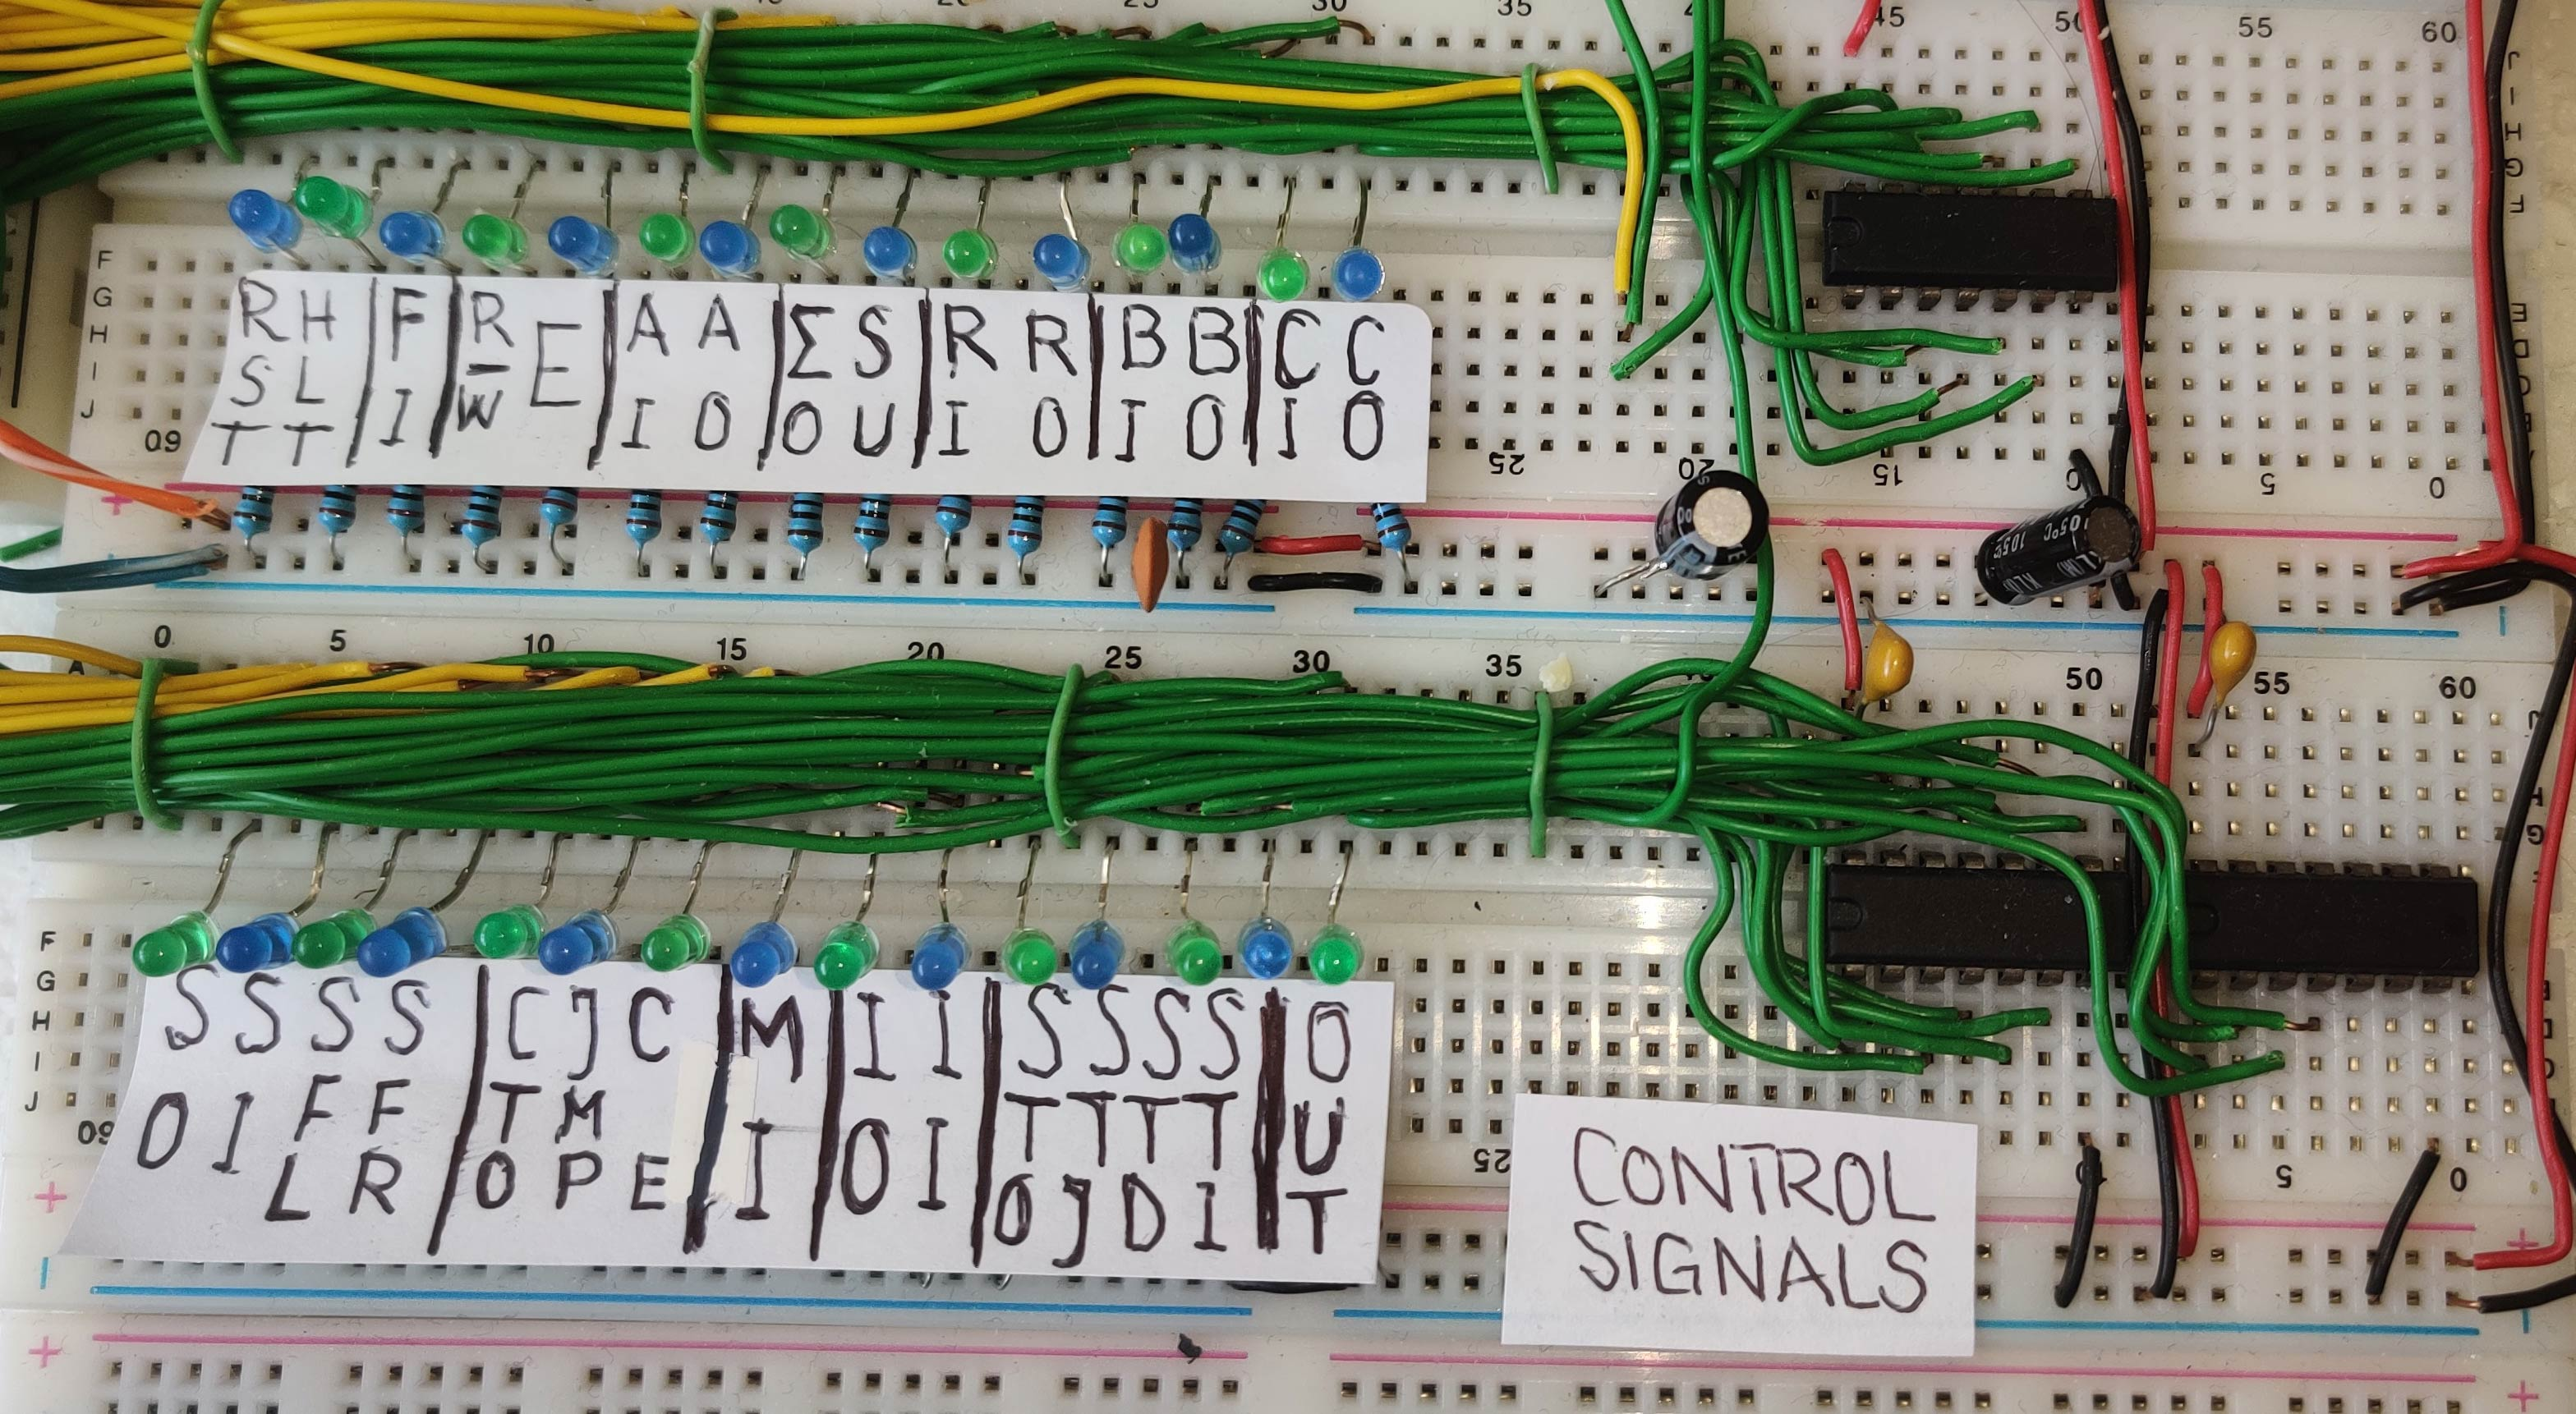
\includegraphics[scale=0.1]{comp/control-sigs}
    \caption{Implementation of the contol signals module}
    \label{control-sigs-i}
  \end{figure}

  \begin{figure}[h]
    \centering
    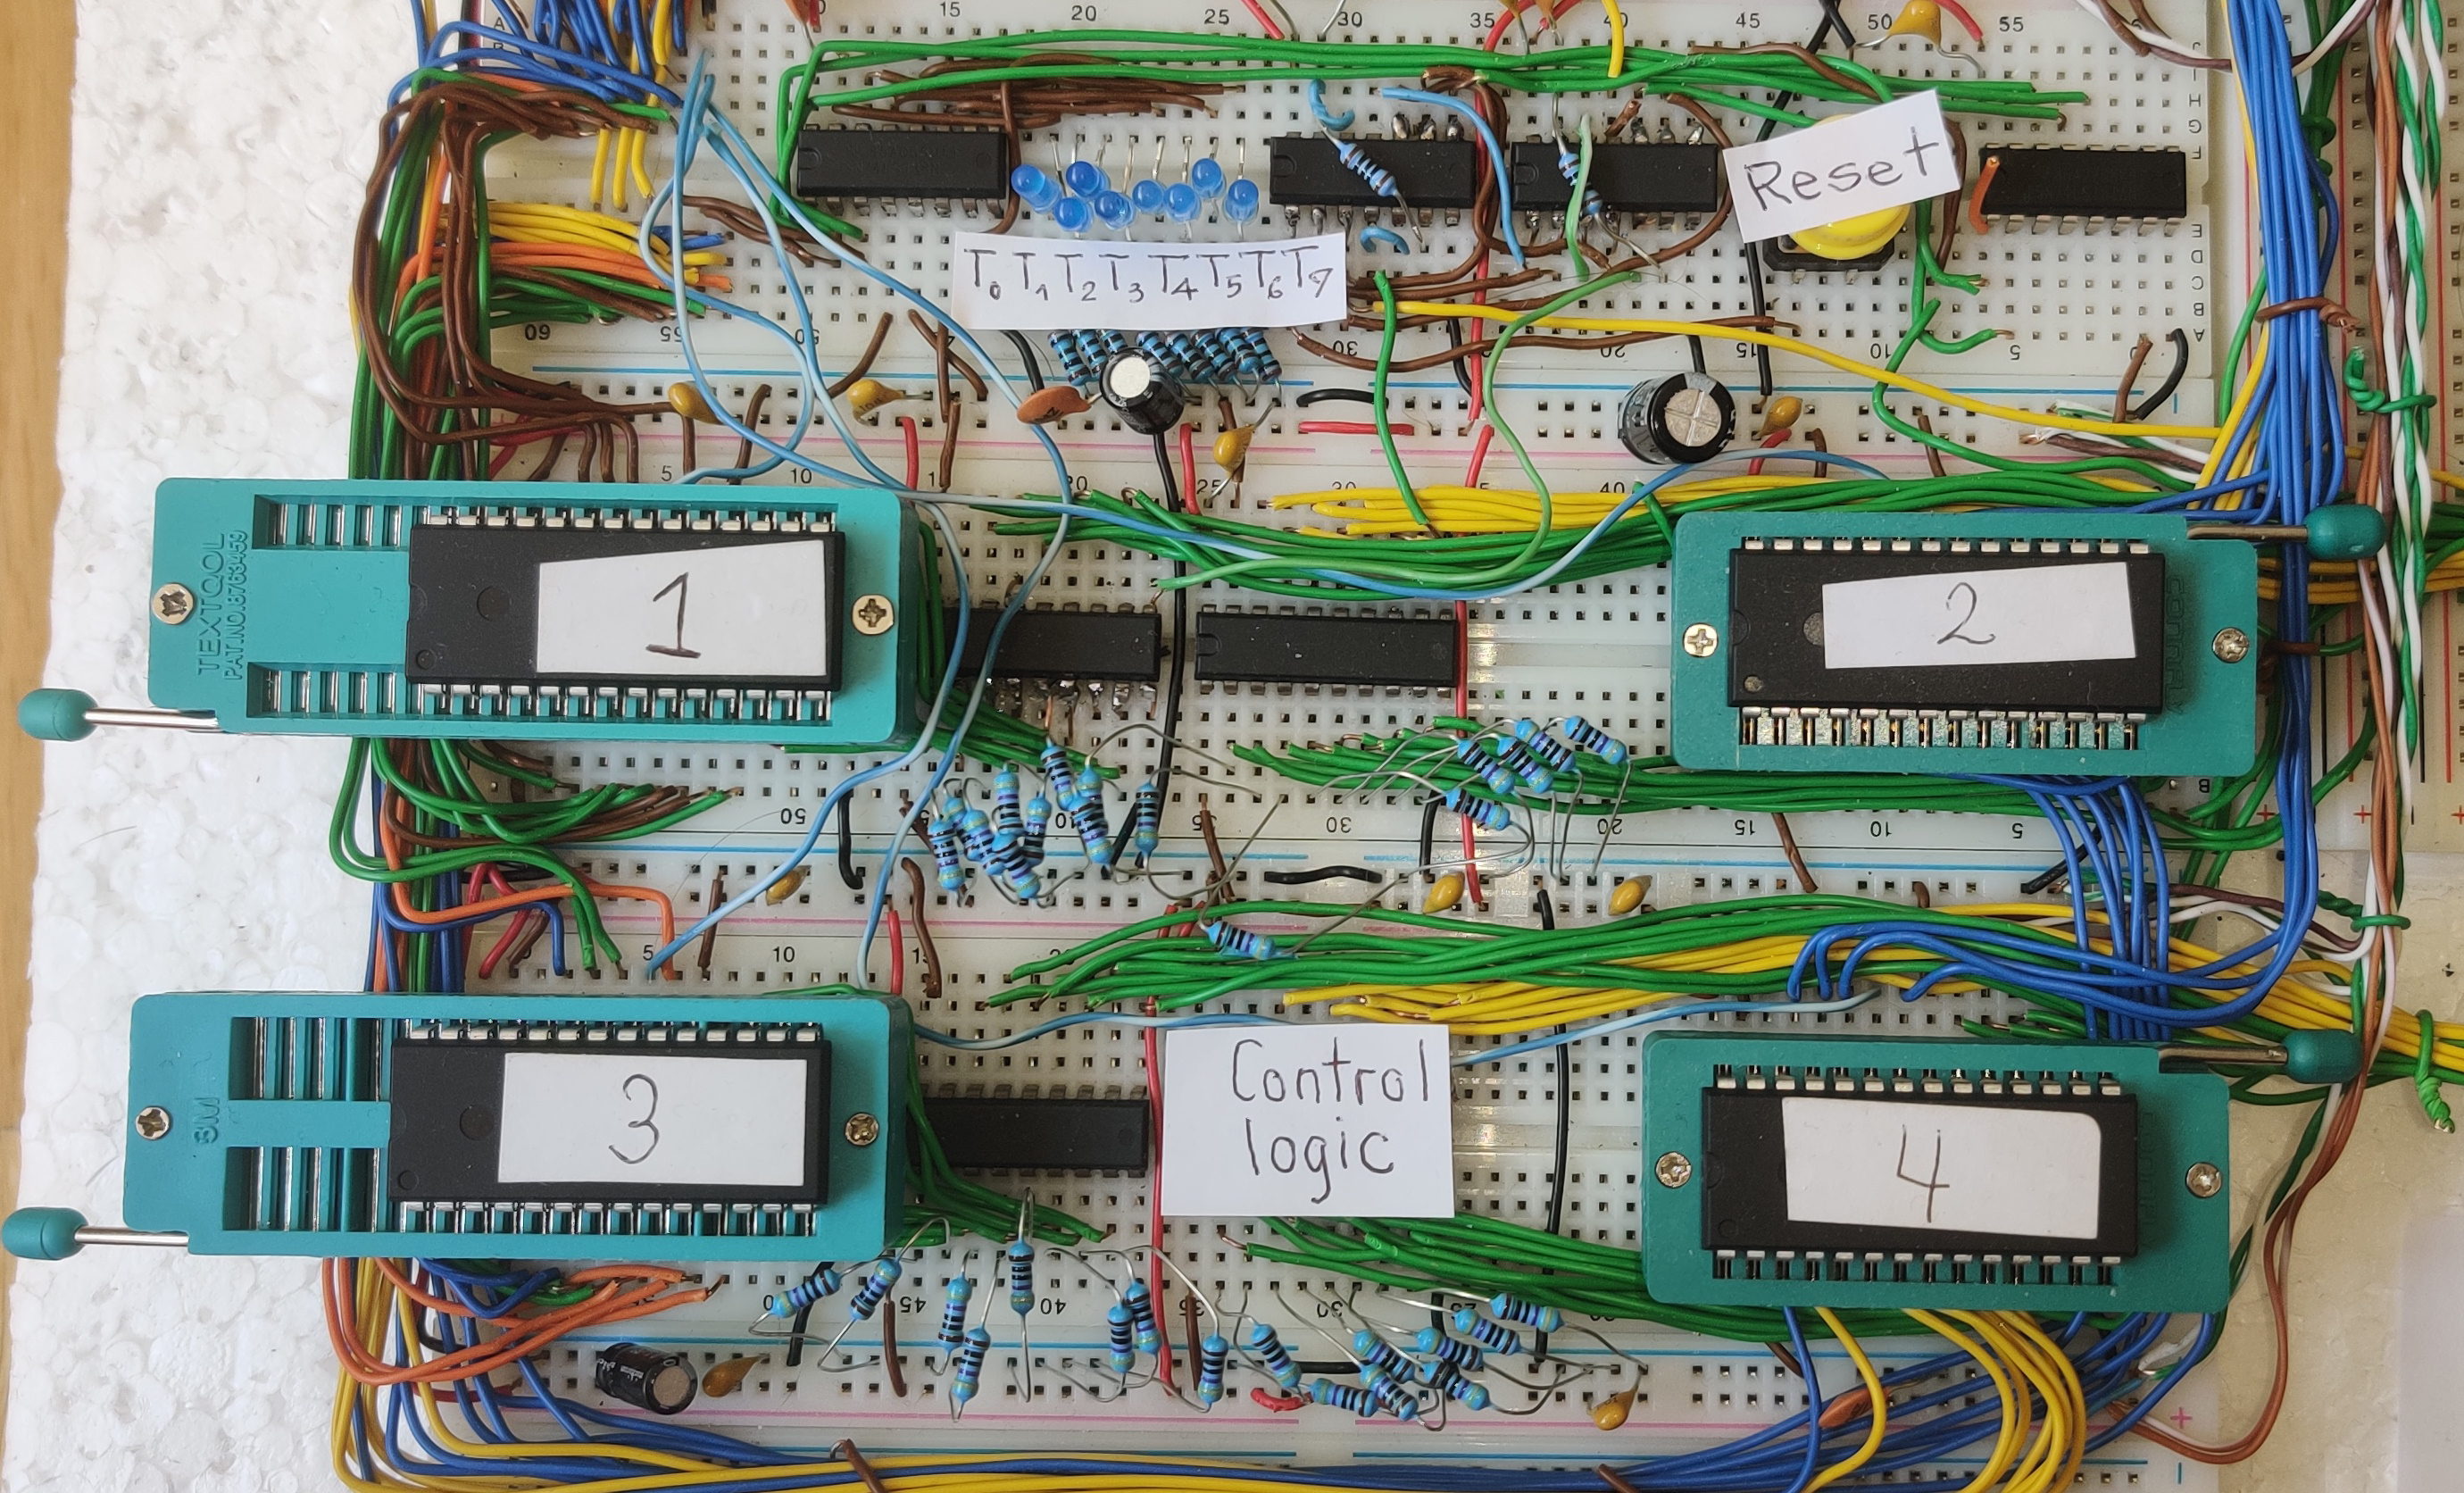
\includegraphics[scale=0.1]{comp/control-logic}
    \caption{Control Logic implementation}
    \label{control-logic-i}
  \end{figure}

  \begin{figure}[h]
    \centering
    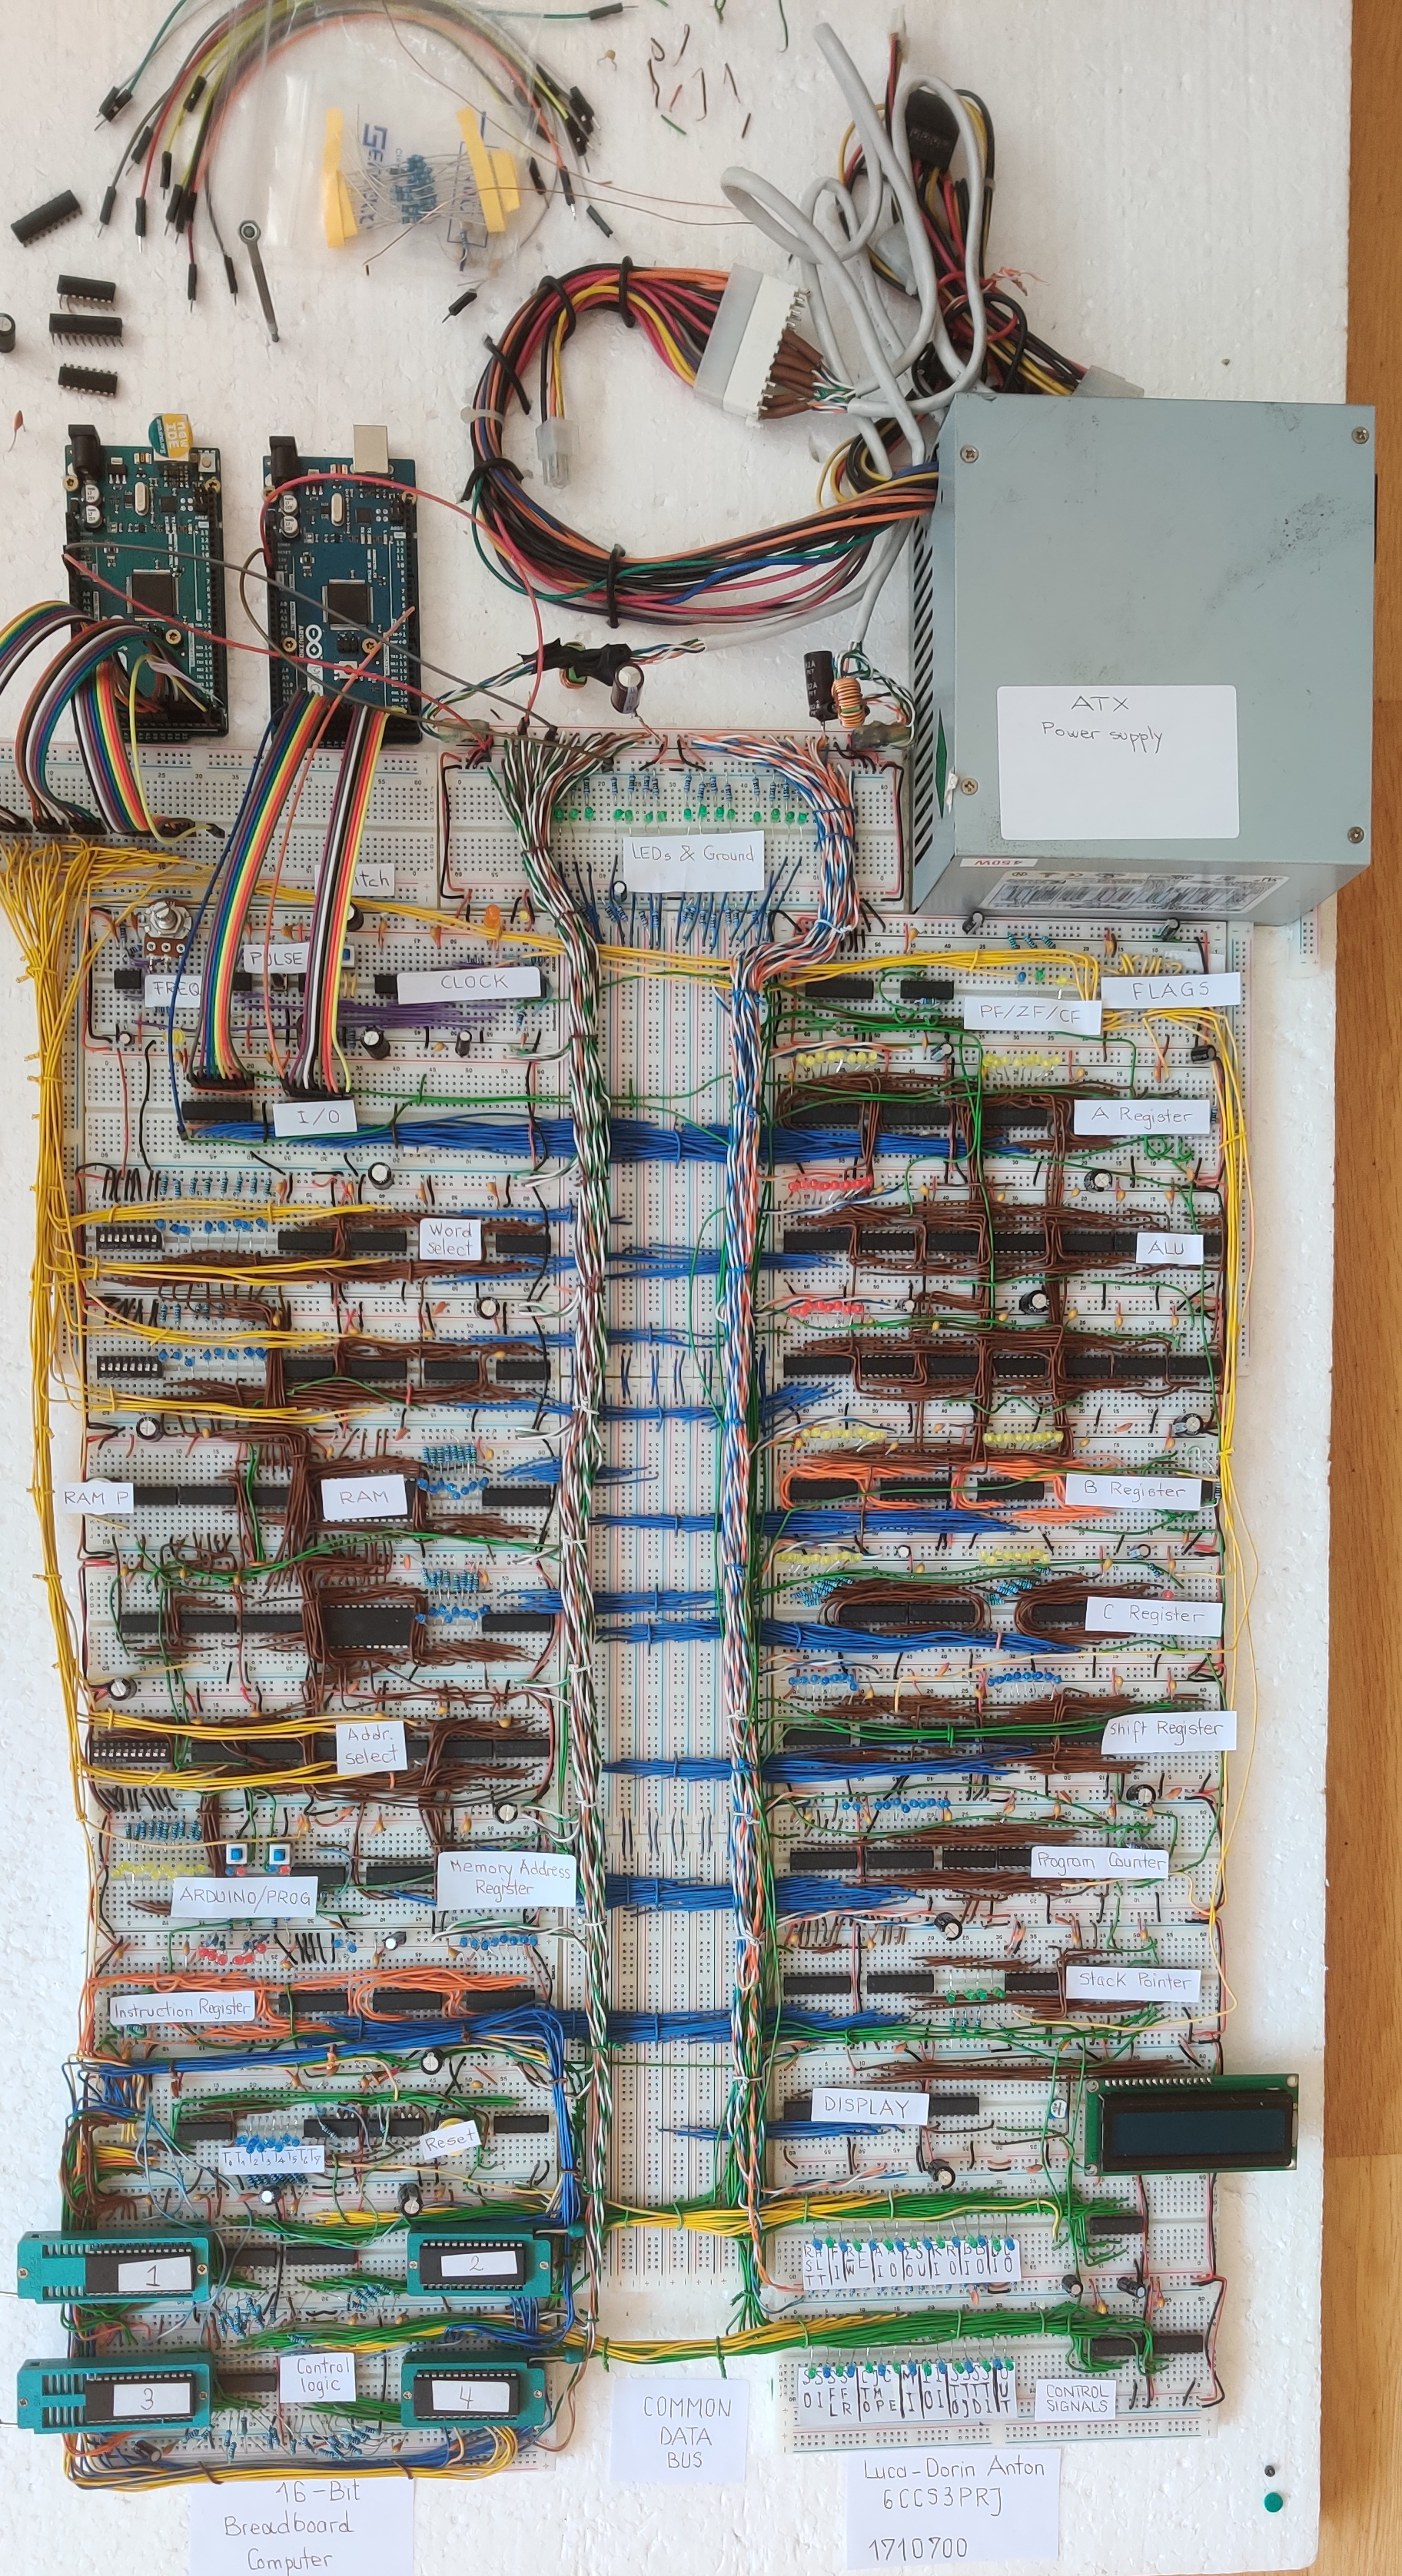
\includegraphics[scale=0.1]{comp/high-level}
    \caption{High level overview (with bus and LEDs visible)}
    \label{high-level-i}
  \end{figure}

\cleardoublepage
\cleardoublepage

\chapter{Source Code}
\section{Instructions}
Complete source code listings must be submitted as an appendix to the report. The project source codes are usually spread out over several files/units. You should try to help the reader to navigate through your source code by providing a ``table of contents'' (titles of these files/units and one line descriptions). The first page of the program listings folder must contain the following statement certifying the work as your own: ``I verify that I am the sole author of the programs contained in this folder, except where explicitly stated to the contrary''. Your (typed) signature and the date should follow this statement.

All work on programs must stop once the code is submitted to KEATS. You are required to keep safely several copies of this version of the program and you must use one of these copies in the project examination. Your examiners may ask to see the last-modified dates of your program files, and may ask you to demonstrate that the program files you use in the project examination are identical to the program files you have uploaded to KEATS. Any attempt to demonstrate code that is not included in your submitted source listings is an attempt to cheat; any such attempt will be reported to the KCL Misconduct Committee.

\textbf{You may find it easier to firstly generate a PDF of your source code using a text editor and then merge it to the end of your report. There are many free tools available that allow you to merge PDF files.}




\bibliographystyle{plain}
\bibliography{Appendix}
\addcontentsline{toc}{section}{Bibliography}


\end{document}
